\chapter{Visual Analytics of Microblog Data for Public Behavior Analysis in Disaster Events}

%\textit{Hurricane Sandy} approached Northeastern United States during late October 2012 and New York City announced a mandatory evacuation of some low-lying areas in the morning on October 28th. these three figures show the southern part of Manhattan. (Left) shows spatial user-based Tweet distribution from noon to 4:00 PM, right after the evacuation order. We overlay the locations of big supermarkets (blue pin) on the same heatmap. we see relatively many number of people immediately go to supermarkets. (Center and Right) shows the distributions during one and two weeks before the same time period. The hotspots are locationally much different from ones of (Left). The green pins on the maps, (Center and Right) indicate the locations of big parks in the southern region of Manhattan. The many hotspots overlap with the park areas; this would be a normal situation on Sunday.


%For emergency and disaster management, analysis of public behavior, such as how people prepare and respond to disasters, is important for evacuation planning.
Analysis of public behavior plays an important role in crisis management, disaster response, and evacuation planning. 
As social media has played a pervasive role in the way people think, act, and react to the world (more than 40 million Americans use social media Web sites multiple times a day~\cite{TW:2010:SHF}), social media is changing the way people communicate not only in their daily lives, but also during abnormal events, such as natural disasters.
In emergency situations, people even seek social confirmation before acting in response to a situation, where they interact with others to confirm information and develop a better informed view of the risk~\cite{national:2013:Public}.
A study commissioned by the American Red Cross, found that roughly half of the respondents would mention emergencies and events on their social media channels, and more than two-thirds agree that response agencies should regularly monitor postings on their websites~\cite{ARC:2010:SMD}.
Moreover, a growing number of people are using Location-based Social Network services, such as microblogs, where they create time-stamped, geo-located data and share this information about their immediate surroundings using smart phones with GPS. 
Such spatiotemporal data has great potential for enhancing situational awareness during crisis situations and providing insight into the evolving event, the public response, and potential courses of action. 

%From government agencies and other organizations, to citizens and social platforms themselves, people across the spectrum of social media are leveraging its use to respond to emergencies. 
%According to a 2011 report of the Congressional Research Service, there are two broad categories in the way that we can conceptualize this use of social media: 1) to "somewhat passively" disseminate information and receive user feedback; and 2) to use social media more systematically as an emergency management tool.

%Unfortunately, finding meaningful information for the analysis is challenging and collecting relevant data would create even high cost.

For public behavior analysis in disasters, however, finding meaningful information from social media is challenging. It is almost impossible to perform a straightforward qualitative analysis of the data, since the volume of the data exceeds the boundaries of human evaluation capabilities and normal computing performance.
%since data volume has increased beyond the capabilities of manual evaluations.
Even though we could extract certain information from the data, it is not always easy to determine whether the analysis result of the extracted information is meaningful and helpful.
Thus, there is a need for advanced tools to handle such big data and aid in examining the results in order to understand situations and glean investigative insights.
Given the incomplete, complex, context-dependent information, a human in this analysis and decision-making loop is crucial.
Therefore, a visual analytics approach offers great potential through interactive, scalable, and verifiable techniques, helping analysts to extract, isolate, and examine the results interactively.
In this thesis, we present an interactive visual analytics approach for spatiotemporal microblog data analysis to improve emergency management, disaster preparedness, and evacuation planning~\cite{Chae:2014:Public}.
We demonstrate the ability to identify spatiotemporal differences in patterns between emergency and normal situations, and analyze spatial relationships among spatial distributions of microblog users, locations of multiple types of infrastructure, and severe weather conditions.
Furthermore, we show how both spatiotemporal microblog and disaster event data can help the analysts to understand and examine emergent situations, and evaluate courses of action.
%location-based public behavior and locations of multiple types of infrastructures.


This study is performed using Tweets, as Twitter has been the most popular microblog service in the United States.
We extend our previous work~\cite{Chae:2013:VAM} with additional features of our system and examine their capabilities with several expanded examples in Section~\ref{sec:spatial_decision_support}.
%explain them through more number of case studies (wider range of east coast for the hurricane and a tornado case in the city of Moore) in Section~\ref{sec:spatial_decision_support}.
We also add a discussion section for comparisons and analysis of the case studies.
%that were published before, during, and after 
%hurricane \textquotedblleft Sandy \textquotedblright 
%\textit{Hurricane Sandy}.
%that hit the New York City area on October 29th, 2012.
%For this study, 1,740,114 Tweets published by 92,683 people are used.

Our system evaluates visual analytics of spatiotemporal distribution of Tweets to identify public behavior patterns during natural disasters.
%We propose an approach that visualizes spatiotemporal distribution of Tweets to identify public behavior patterns during natural disasters.
The main features of our approach are as follows:
\begin{itemize}
	\item \textbf{Spatial analysis and decision support:} The system provides effective analysis for exploring and examining the spatial distribution of Twitter users and supporting spatial decision-making using a large volume of geo-located Tweets and multiple types of supplementary information during specific time periods (i.e., disaster events).
\item \textbf{Temporal pattern analysis:} Our visualization system enables the analysts to analyze the temporal distribution of the number of Twitter users posting Tweets in a given location and time.
\item \textbf{Spatiotemporal visualization:} We provide a visualization that allows the analysts to simultaneously analyze both aspects: space and time in a single view.
\end{itemize}

%We first review previous work in Section 2 and describe
%our interactive analysis system in Section 3. 
%We present analysis results for two natural disaster events in Section 4
%and discussion in Section 5. Finally conclusion and future directions are presented
%in Section 6.

\section{Problem Statement and Interactive Analysis Process Design}
\label{sec:analysis_process}
Analysis of public behavior, such as how people prepare and respond to disasters, plays an important role in crisis management, disaster response, and evacuation planning. 
Recently, social media becomes popular and people utilize it for communications not only in their daily lives, but also in abnormal disastrous situations.
Thus, Location-based Social Networks services offer a new opportunity for enhancing situational awareness during disaster events.
Unfortunately, collecting relevant data can be costly and finding meaningful information from the huge volume of social media data is very challenging.
%However, the huge volume of the data is another challenging issue in analyzing and evaluating the data.
Therefore, there is a need for an advanced tool to analyze such massive (\textquotedblleft big\textquotedblright) streaming data and aid in examining the analysis results to better understand situations more efficiently.

\begin{figure}[tb]
%\centering
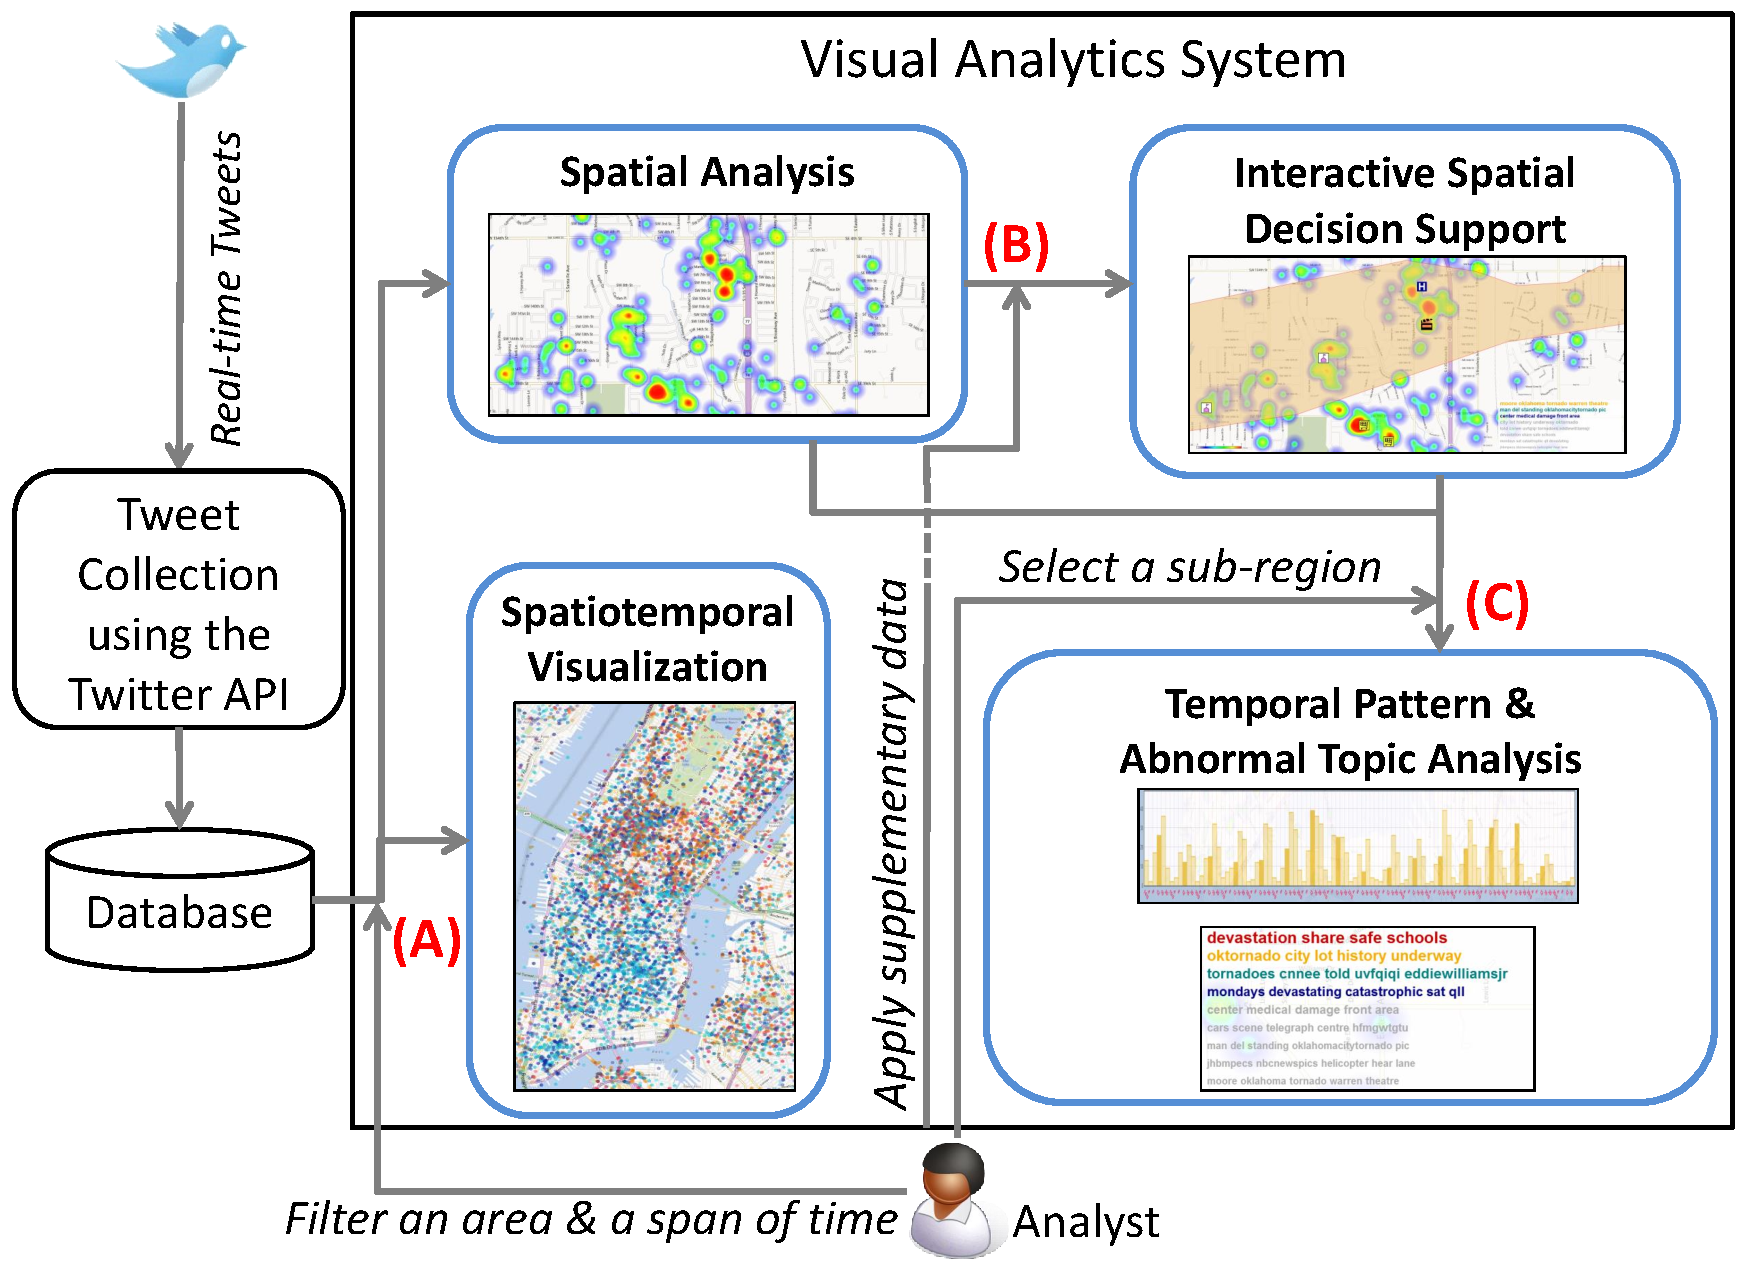
\includegraphics[width=1.0\linewidth]{System_v7}
\caption{Overview of our interactive analysis scheme for public behavior analysis using social media data.}
\label{fig:analysis_process}
%\vspace{-0.4cm}
\end{figure}

Our proposed visual analytics approach provides multiple analysis methods: spatial analysis, spatial decision support, temporal pattern analysis, abnormal topic analysis, and interactive spatiotemporal visualization as shown in Figure~\ref{fig:analysis_process}.
In our system, all methods are tightly integrated based on a user-centered design in order to enhance the ability to analyze huge social media data (Figure~\ref{fig:analysis_process}~(A, B, C)).
Our Tweet collection component obtains real-time Tweets using the Twitter API\textemdash to collect about 2.2 million geotagged Tweets within the United States per day.
In general for spatial analysis, the required accuracy of the geocoordinate depends upon the required level of location granularity.
The data, however, is generated by very reliable GPS and software.
%We can be reasonably certain about their accuracy
We can be reasonably certain about the data accuracy as illustrated in~\cite{TWITTER:2013:GOT}.
For the temporal accuracy of Tweets, we use the time when each Tweet is created. 
Therefore, it is highly accurate if the time setting of the device posting a Tweet is correct.
This large volume of data is stored in our database in order to maintain and track the history of the Twitter stream.
%The analyst can select an area and a timespan to be analyzed.
Our system allows the analysts to query Tweets with a specific area and time span condition (Figure~\ref{fig:analysis_process}~(A)).
%The initially selected spatiotemporal context of Twitter messages is represented by two different analytics components, such as spatial analysis and spatiotemporal visualization.
The initially selected spatiotemporal context of Tweets can be represented by two different analytics components: spatial analysis and spatiotemporal visualization.
Spatial analysis allows the analysts to examine the overall distribution of Twitter users and discover hotspots where relatively more Twitter users post Tweets.
The analysts are able to add supplementary information (infrastructure locations, tornado paths) on top of current information representing outcomes in order to better understand events and increase situational awareness (Figure~\ref{fig:analysis_process}~(B)).
Furthermore, the analysts can select a sub-region within the initial area, so that he can analyze the temporal patterns of the number of Twitter users and extract abnormal topics from the text messages in the selected region (Figure~\ref{fig:analysis_process}~(C)).
In addition, our interactive spatiotemporal visual analytics provides a single view representation for the analysis of both aspects: spatial and temporal characteristics of Tweets at the same time.


\section{Spatiotemporal Analysis}
\label{sec:body}

%Since many social media channels provide time-referenced geographic data, traditional techniques for spatiotemporal zooming and filtering can easily be applied to explore social media data.
%However, as the volume of the data exceed the boundaries of human evaluation capabilities and even normal computing performance, it is almost impossible to perform a straightforward qualitative analysis of the data.
%Therefore, the task for examining and determining whether the extracted result is meaningful is still challenging.
%In order to address the issues, traditional visualization approaches have to be enhanced with more interactive, scalable, and verifiable techniques, helping analysts to extract, isolate, and examine the results interactively.
In this work, we present a visual analytics approach to handle the vast amount of microblog data such as Twitter messages, provide interactive spatiotemporal analysis, and enable the use of multiple types of supplementary spatial infrastructure information for spatial decision support.
%combinational analysis of social media with different types of spatial data 
Analysts select an initial spatiotemporal context of Tweets to be represented in the visualization to serve as a basis for analysis. 
They can also perform the interactive spatiotemporal queries that load the relevant datasets from a larger database.

%in order to examine and verify the results.
%For the public behavior analysis in disasters, however, finding meaningful information from social media is challenging, since data volumes have increased beyond the capabilities of manual evaluation.
%Even though we extract certain information from the data set, it is not always easy to determine whether the result is meaningful.
%Thus, there is a need for advanced tools to handle such big data and even aid in examining the results in order to understand the situations and glean investigative insights.
%In this paper, we present an interactive visual analytics tool for spatiotemporal social media data analysis to improve emergency management, disaster preparedness and evacuation planning by allowing to identify spatiotemporal differences between emergency and normal situations, and analyze spatial relationship between location-based public behavior and locations of multiple types of infrastructures.




\subsection{Spatial Analysis}
\label{sec:spatial_analysis}
%
Social media embedding geo-location information into the data is extremely useful in analyzing location-based public behaviors.
Such spatial analysis, therefore, is important in order to manage and prepare plans for disaster and emergency situations.
%The spatial characteristics together with heterogeneous information can assist in disaster management and migrating hazards where the problems have spatial components~\cite{Andrienko:2007:GAS}.
%In this section, we present how our system supports spatial decision-making by combining different types spatial data: location-based microblog data and spatial infrastructure data.

\begin{figure}[htb]
\centering
%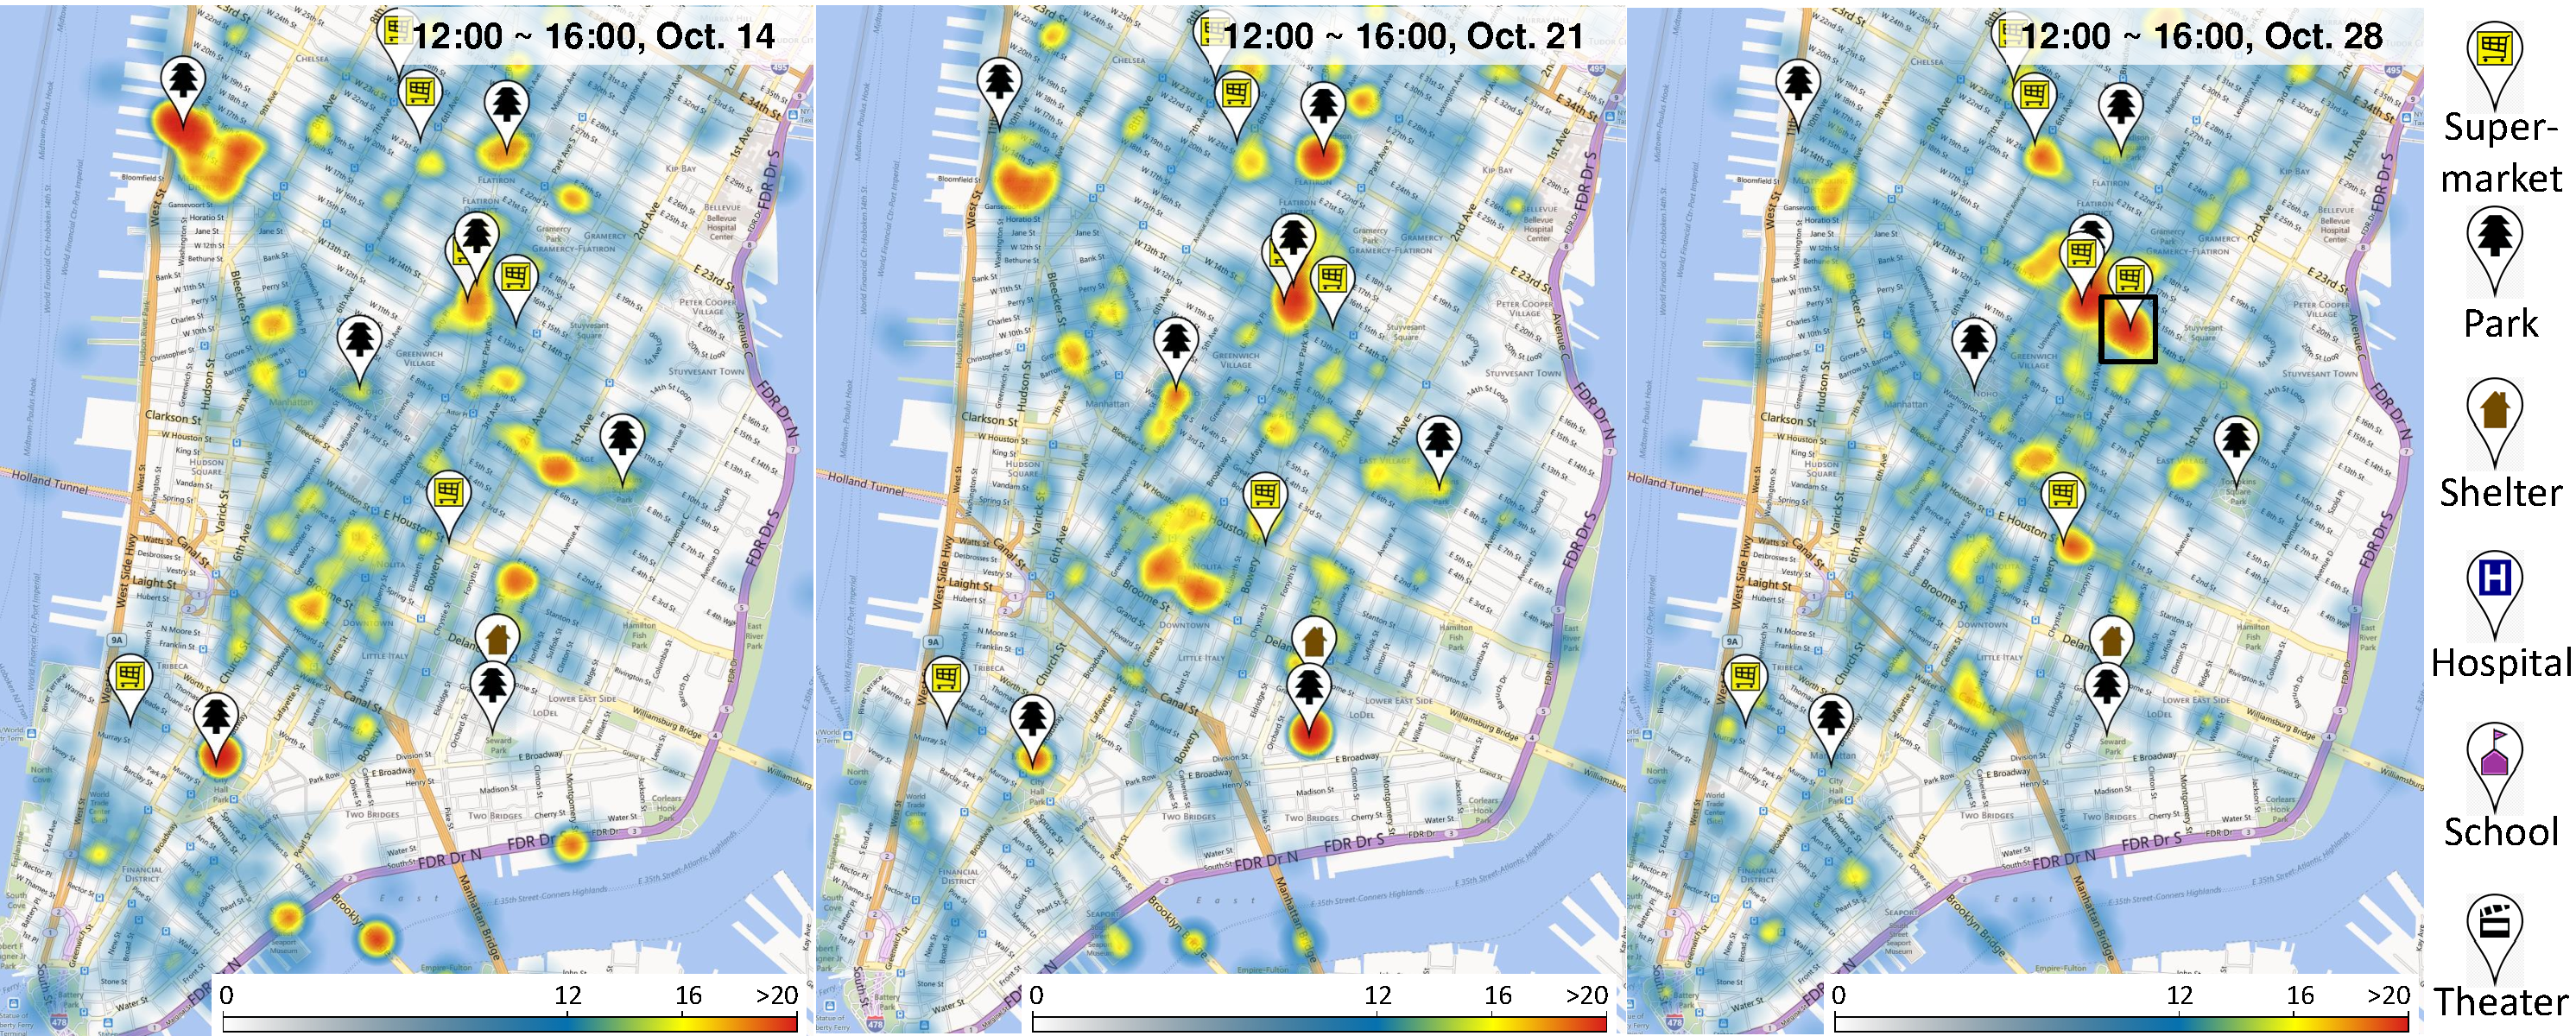
\includegraphics[width=0.9\linewidth]{heatmap_manhattan_v3}
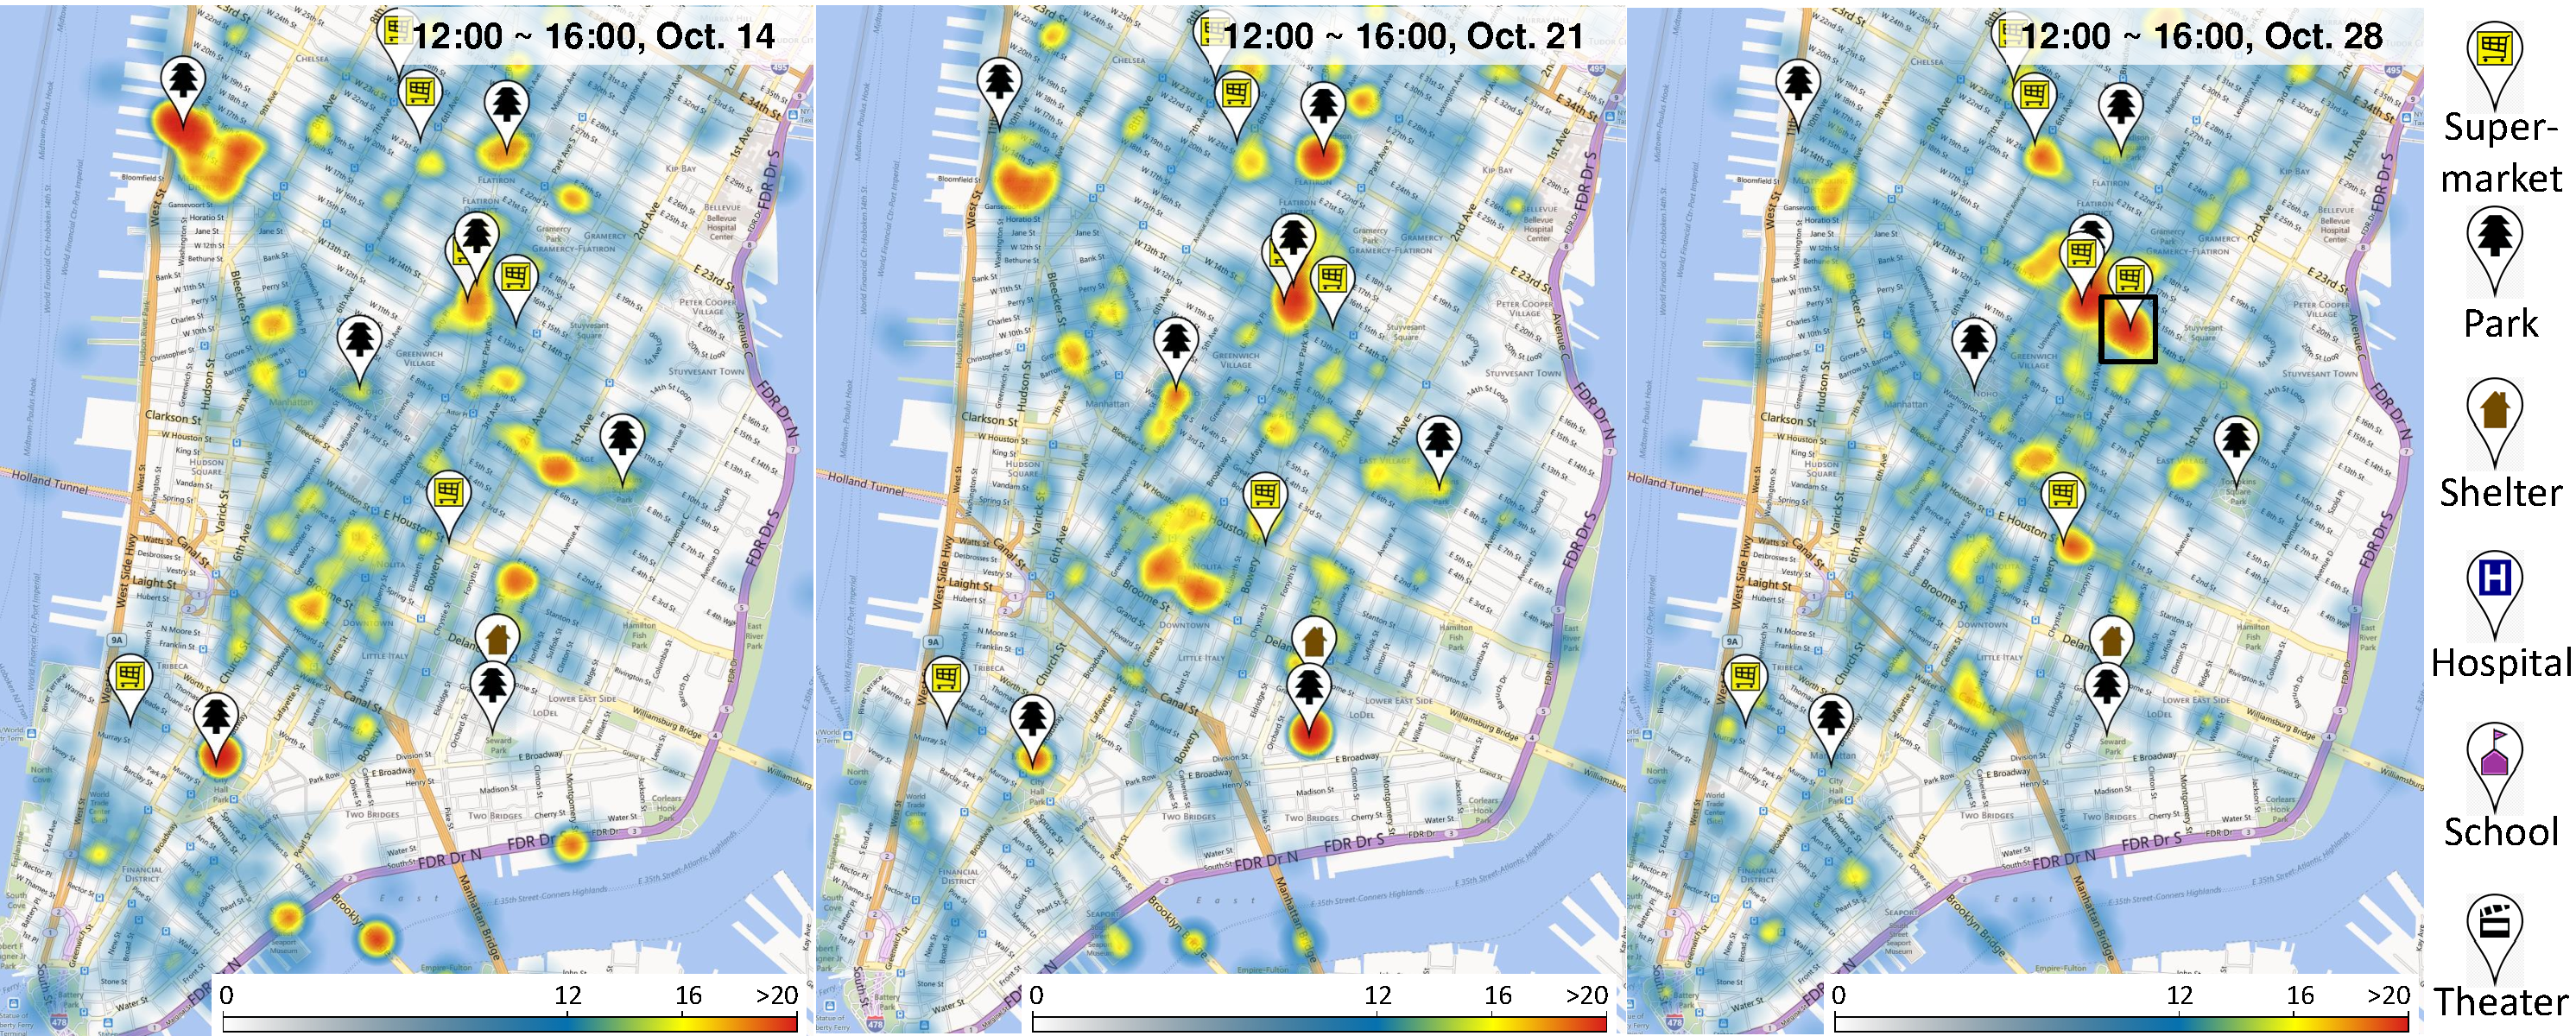
\includegraphics[width=1.0\linewidth]{heatmap_manhattan_v3}
\caption{Spatial user-based Tweet distribution in the Manhattan area in New York City during four hours right after the evacuation order (from 12:00 PM to 4:00 PM on October 28th, 2012 (Right)). Previous distribution of Tweets on 14th (Left) and 21st (Center).}
\label{fig:heatmap_manhattan}
%\vspace{-0.4cm}
\end{figure}

In late October in 2012, a massive hurricane, Sandy, devastated Northeastern United States~\cite{WKP:2012:SANDY}.
Due to the severeness of the hurricane,  on October 28th in 2012, the New York City Authorities ordered residents to leave some low-lying areas\textemdash the mandatory evacuation zones (red color) are shown in Figure~\ref{fig:spatiotemporal} (Right).
%Shelters were opened in the morning on October 28th ahead of the storm approaching the eastern third of the United States \-- the mandatory evacuation zones (red color) are shown in Figure~\ref{fig:spatiotemporal} (Right).
We investigate an area of Manhattan, since the area is the most populated and severely damaged.
Through the map view in our system, analysts navigate to the Manhattan area in New York City and filter Tweets posted within the area. 
%appearing in the view during two weeks before and after October 28th.
Initially we tried to reveal public movement flows during the disaster event, but the movement patterns were too complicated to find meaningful flows due to movement randomness and the visual clutter of the flows.
Then, we examined the spatial distribution of the users for specific time frames.
Based on our experiments, a geospatial heatmap was useful for an overview of the spatial distribution and for trend approximation.
We utilize a divergent color scheme to generate the heatmap, where saturated colors are used for the data distribution to avoid any confusion from the color scheme from the desaturated colormap of the background map.
Analysts can specify a threshold range to emphasize hotspots, where the upper bound is mapped to a red color and the lower bound to a yellow color.
Additionally, the blue color is mapped by the analysts to the value of the overall distribution of Twitter users.
In Figure~\ref{fig:heatmap_manhattan}, we show three heatmaps of spatial user-based Tweet distribution from 12:00 PM to 4:00 PM on October 14th (Left), 21st (Center), and 28th (Right).
In this work, we use the number of Twitter users instead of the number of Tweets for the heatmap generations to properly reflect the flow of evacuation unbiased by personal Tweet activity or behavior of individual users, since some enthusiastic Twitter users generate a large number of Tweets at the same location during a short time period (more than 20 Tweets per hour).
The heatmaps in Figure~\ref{fig:heatmap_manhattan} (Left and Center) represent normal situations of Twitter user distribution in the Manhattan area, and the heatmap (Right) shows the situation right after the evacuation order that was announced at 10:30 AM on October 28th, 2012.
This standard heatmap visualization allows analysts to explore the spatial pattern of Twitter users for any specified time period.
In Section~\ref{sec:spatial_decision_support}, we will provide further analysis for the spatial decision support.

\begin{figure}[tbh]
\centering
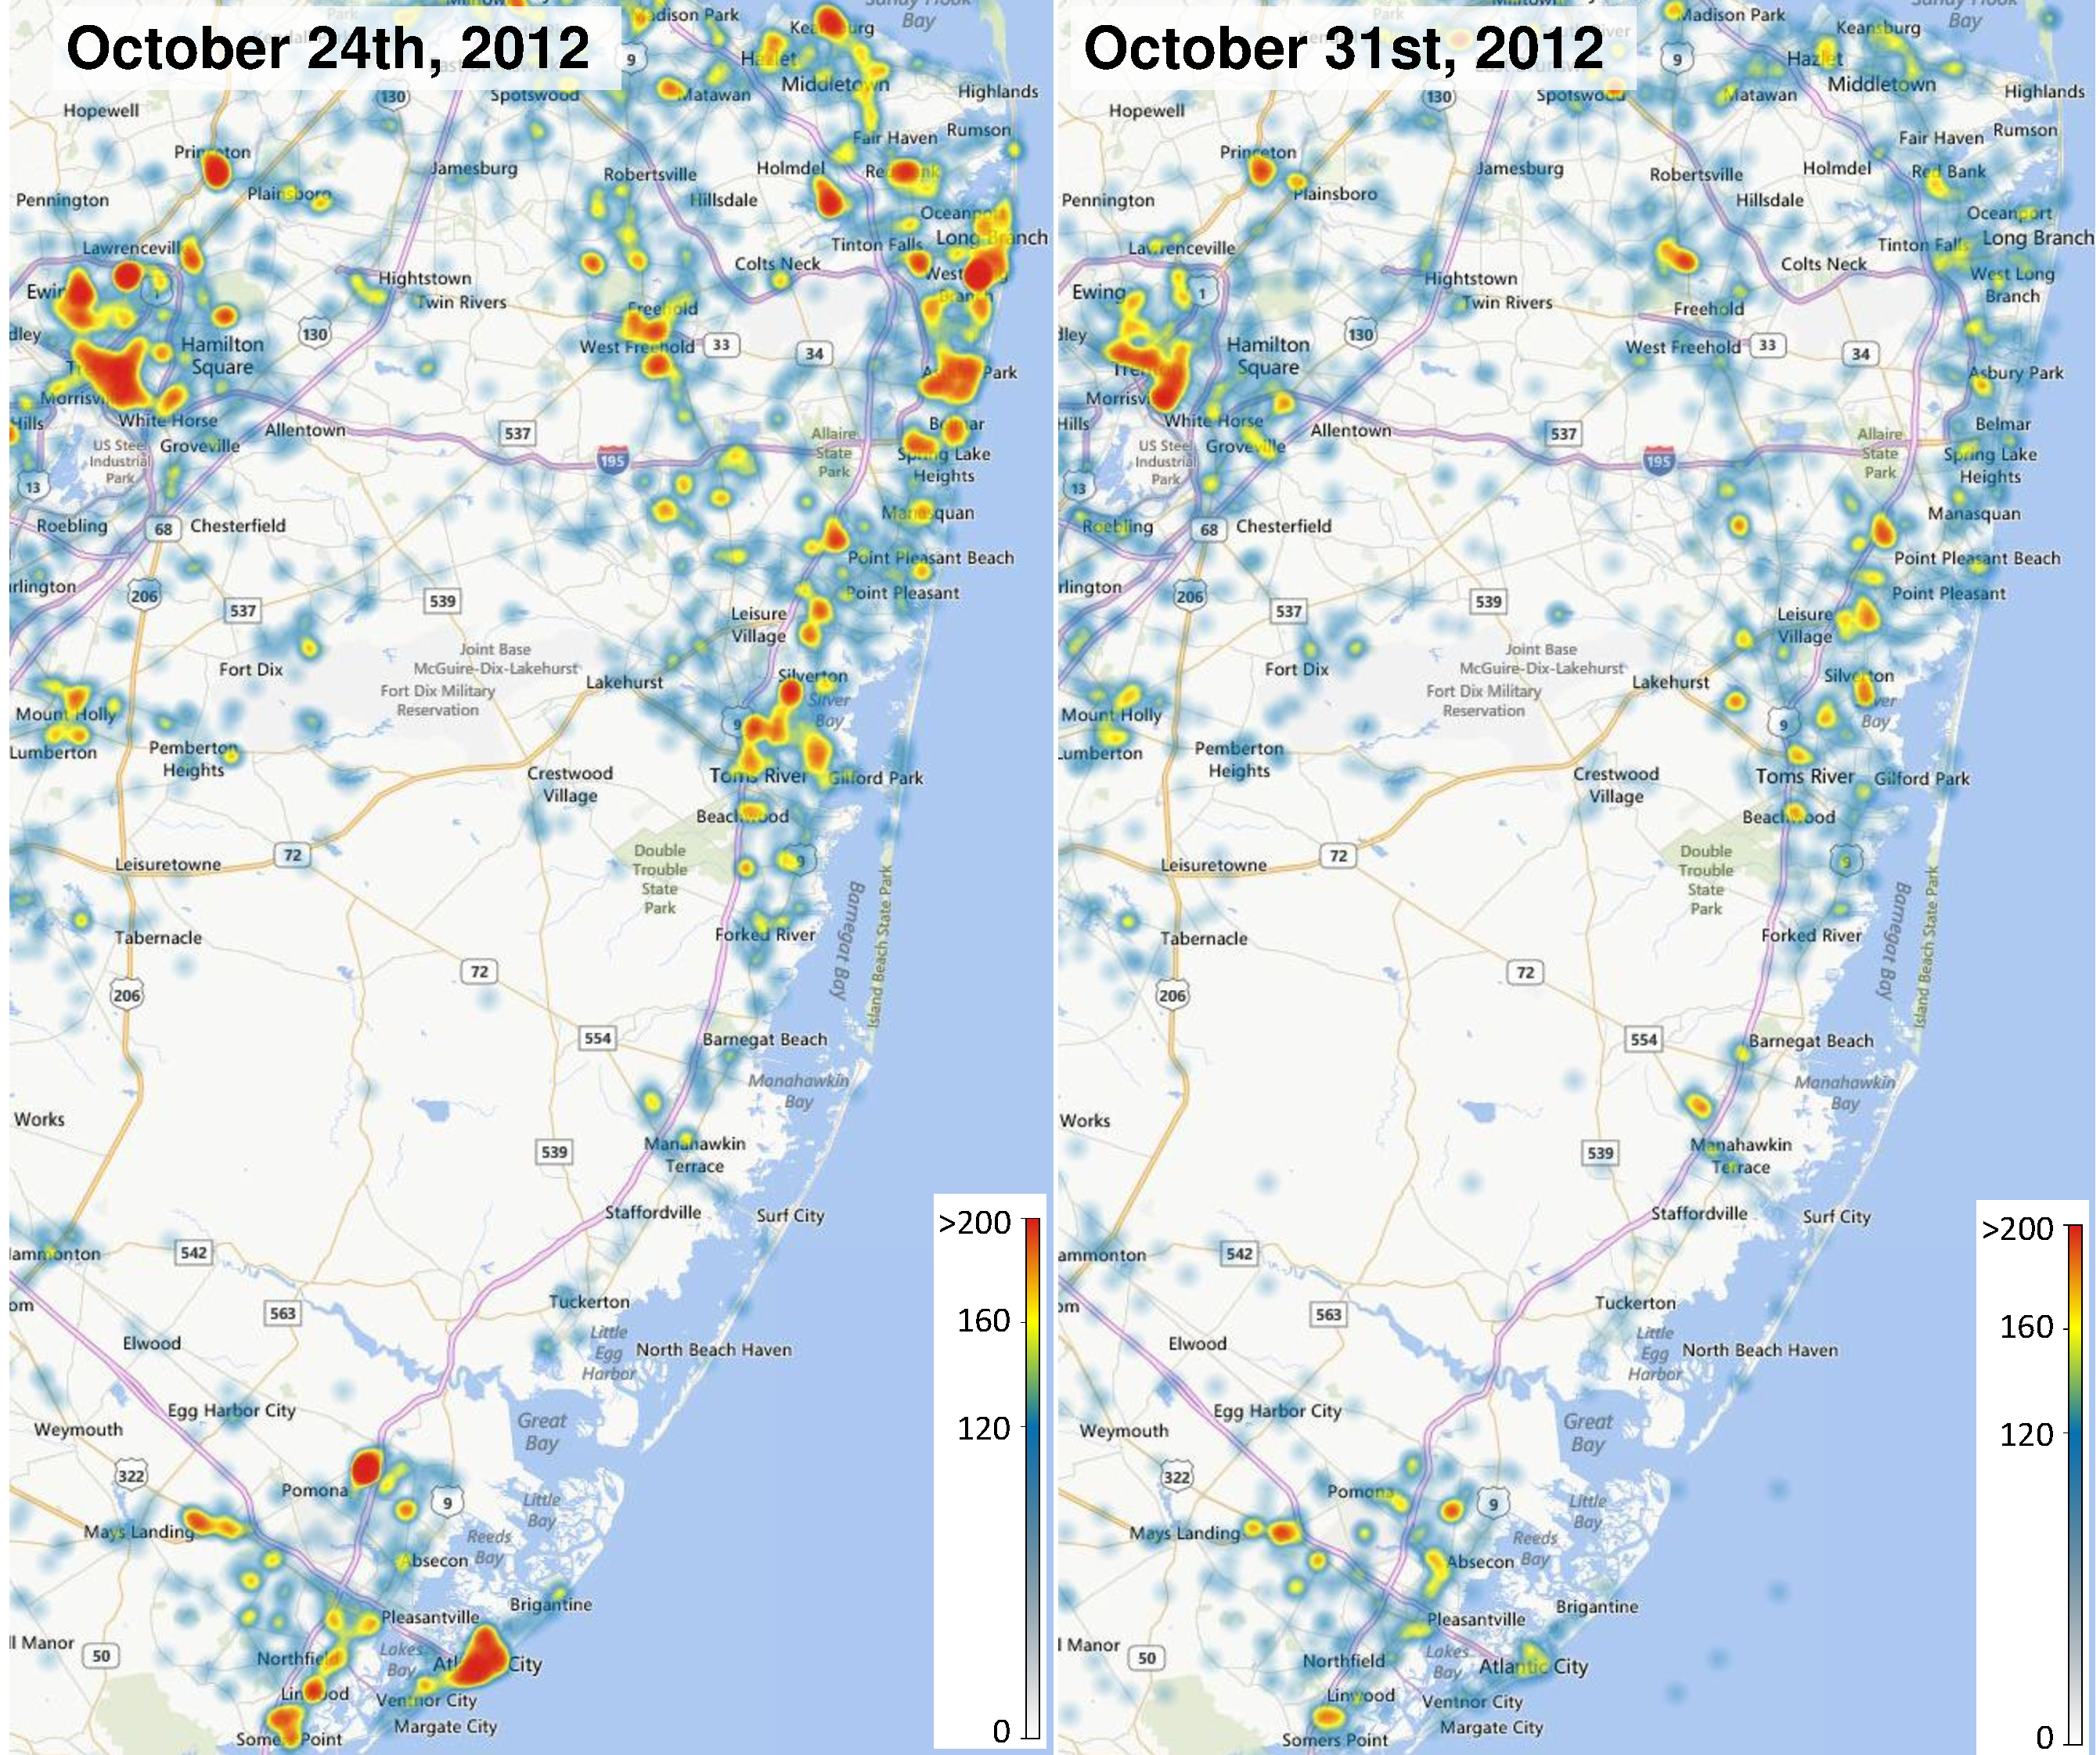
\includegraphics[width=1.0\linewidth]{Atlantic_Coast_v6}
\caption{Twitter user distribution on the eastern coast area in New Jersey, after the hurricane passed over the area on October 31st (Right). Previous distribution on October 24th is shown on the Left.}
\label{fig:atlantic_coast}
%\vspace{-0.4cm}
\end{figure}

Hurricane Sandy damaged not only New York City, but also the entire eastern coast area of New Jersey. 
Most cities in the area also announced evacuation orders on October 28th, 2012.
The distribution of Twitter users in the area from Atlantic City to the upper eastern shore area for two different dates are shown in Figure~\ref{fig:atlantic_coast}.
The heatmaps in Figure~\ref{fig:atlantic_coast} (Left) represent the previous normal situation of Twitter user distribution on October 24th and the heatmap (Right) shows the post distribution after Sandy passed over the area on October 31st.
As shown in the result, many hotspots are gone or diminished.
This situation shows that the number of Twitter users had significantly decreased after the hurricane damaged the area.
In fact, a huge number of homes were damaged or destroyed and a couple of million households lost power because of Hurricane Sandy~\cite{WKP:2012:EHS}.
In disaster management this type of visualization can support analysts estimating which areas were highly damaged and even which areas still need reconstruction.



%
%\begin{figure}[tb]
%\centering
%\includegraphics[width=0.8\columnwidth]{symbols}
%\caption{Standard symbols for infrastructures used in the paper~\cite{Robinson:2012:DMS}.}
%\label{fig:symbols}
%\vspace{-0.5cm}
%\end{figure}
%
%
%




\subsection{Spatial Decision Support}
\label{sec:spatial_decision_support}
%Investigating and making decisions using only the heatmap without any supplementary information are demanding and hard to unserstand the actual events.
In Section~\ref{sec:spatial_analysis}, we introduced our spatial analysis to explore the Twitter user distribution.
In addition to the analysis, our system allows the analysts to utilize supplementary information in order to support understanding of the situations and decision-making in disaster management.
The spatial characteristics together with heterogeneous information can assist in disaster management and migrating hazards where the problems have spatial components~\cite{Andrienko:2007:GAS}.
The supplementary information can be various types of infrastructures (i.e., school, park, supermarket, and shelter), as well as spatial information of disaster events (i.e., hurricane path and damage area of a tornado).
In this section, we describe how our system supports spatial decision-making by correlating such spatial information with location-based microblog data.

\subsubsection{Infrastructure Data}
\label{sec:infrastructure_data}
%
During a natural disaster event, such as Hurricane Sandy, analysts would assume that many people might want to go to the supermarket before staying or evacuating, but they would need supporting evidence before making appropriate decisions and plans.
With our system support, the analysts can simply overlay the locations of large supermarkets on the heatmap of the Twitter user distribution.
The infrastructure locations are indicated by standard symbols~\cite{Robinson:2012:DMS} as 
shown on the right side of Figure~\ref{fig:heatmap_manhattan}.
%presented in Figure~\ref{fig:symbols}.
%(e.g., \textit{Trader Joe's} and \textit{Whole Foods Market}).
%Note that there is no major retail chains, such as Walmart and Target in Manhattan.
A relatively large number of people immediately went to supermarkets nearby the evacuation area, instead of the emergency shelter as shown in Figure~\ref{fig:heatmap_manhattan} (Right).
However, October 28th was Sunday and many people generally would go for grocery shopping on Saturday or Sunday; therefore, the analysts might need to verify whether the heatmap shown in the figure is a normal periodic situation.
The analysts can investigate new Twitter user distributions for different time frames by simply manipulating the time context.
In Figure~\ref{fig:heatmap_manhattan} (Left and Center), we show two distributions for one and two weeks before the disaster period respectively.
Here, we see that the hotspot locations are very different from the ones for October 28th shown in Figure~\ref{fig:heatmap_manhattan} (Right).
For further analysis, we can explore another popular Sunday location\textemdash large parks\textemdash by superimposing the locations on each heatmap.
%, since we can expect that parks would be populated on Sunday.
As shown in Figure~\ref{fig:heatmap_manhattan} (Left and Center), many hotspots overlap with the park areas in normal situations.
Therefore, we can conclude that the situation on October 28th is an unusual non-periodic pattern.
%
%This system can support the analysts to understand the unusual movement patterns and plan resource allocation accordingly for such emergency events.
%
%can realize that the situation on October 28th is unusual and non-periodic. 
%This system can support them to make plans for preparing some responses for the emergency events.



\subsubsection{Disaster Event Data}
\label{sec:event_data}
%
In Section~\ref{sec:infrastructure_data}, we explained how the infrastructure data help the analysts to understand and examine the emergent situations.
During severe weather conditions, people tend to be sensitive to the dynamic variance of the weather conditions.
Relationship analysis, therefore, between the public responses and the spatiotemporal pattern of the severe weather is important.
Our system overlays geographic information of disaster events, for example, center positions and tracks of a hurricane, and damaged areas by a tornado, in order to provide further analysis.
Two case studies are presented as follows:

\textbf{Track of Hurricane:} Figure~\ref{fig:east_coast}~(1) and (2) show the southeastern coast areas of the United States, whereas,
Figure~\ref{fig:east_coast}~(3), (4), and (5) show the northeastern coast areas.
In the figures the distributions of Twitter users for each consecutive date, from October 26th to 30th, 2012, are presented 
using the heatmap visualizations.
We use the number of Twitter users who posted Twitter messages containing one of the following keywords: \textit{hurricane, storm}, and \textit{sandy} in order to analyze Tweets that are highly related to Hurricane Sandy.
Note that Hurricane Sandy reached the southeastern Florida coast on October 26th and passed, then, over the northeastern coast on October 30th, 2012~\cite{WKP:2012:SANDY}.
As shown in Figure~\ref{fig:east_coast}, our system is able to overlay the track of the hurricane on the map.
% according to a time period of interest.
%(the texts on the map were manually added).
The blue pins and the blue lines represent the center locations of the hurricane and its path respectively.

\begin{figure}[tbh]
\centering
%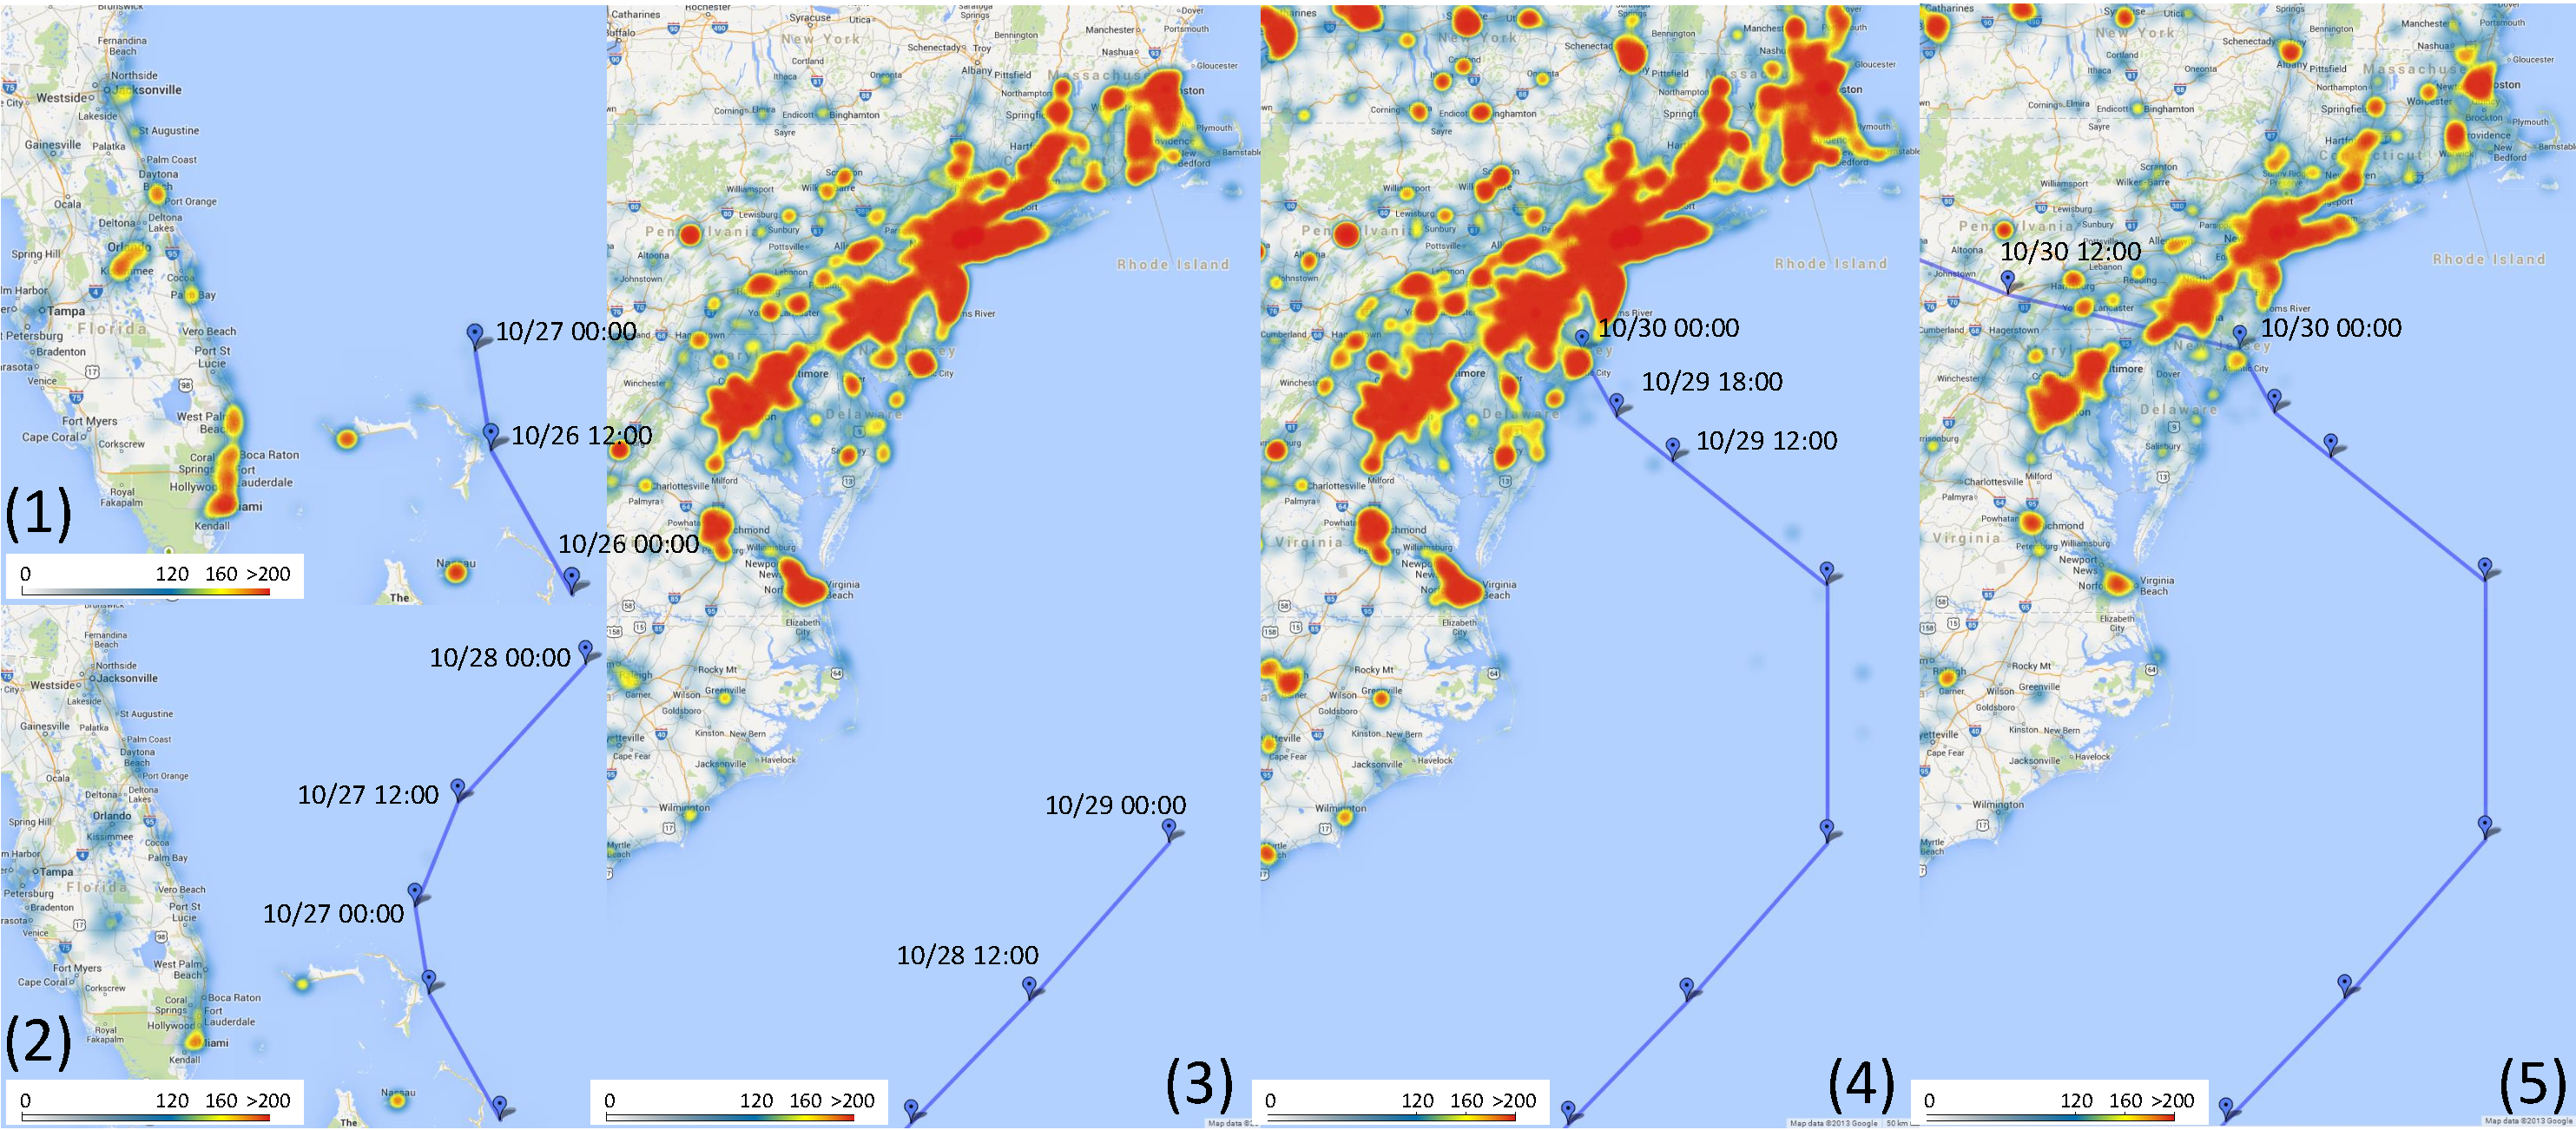
\includegraphics[width=0.85\linewidth]{East_Coast_v7}
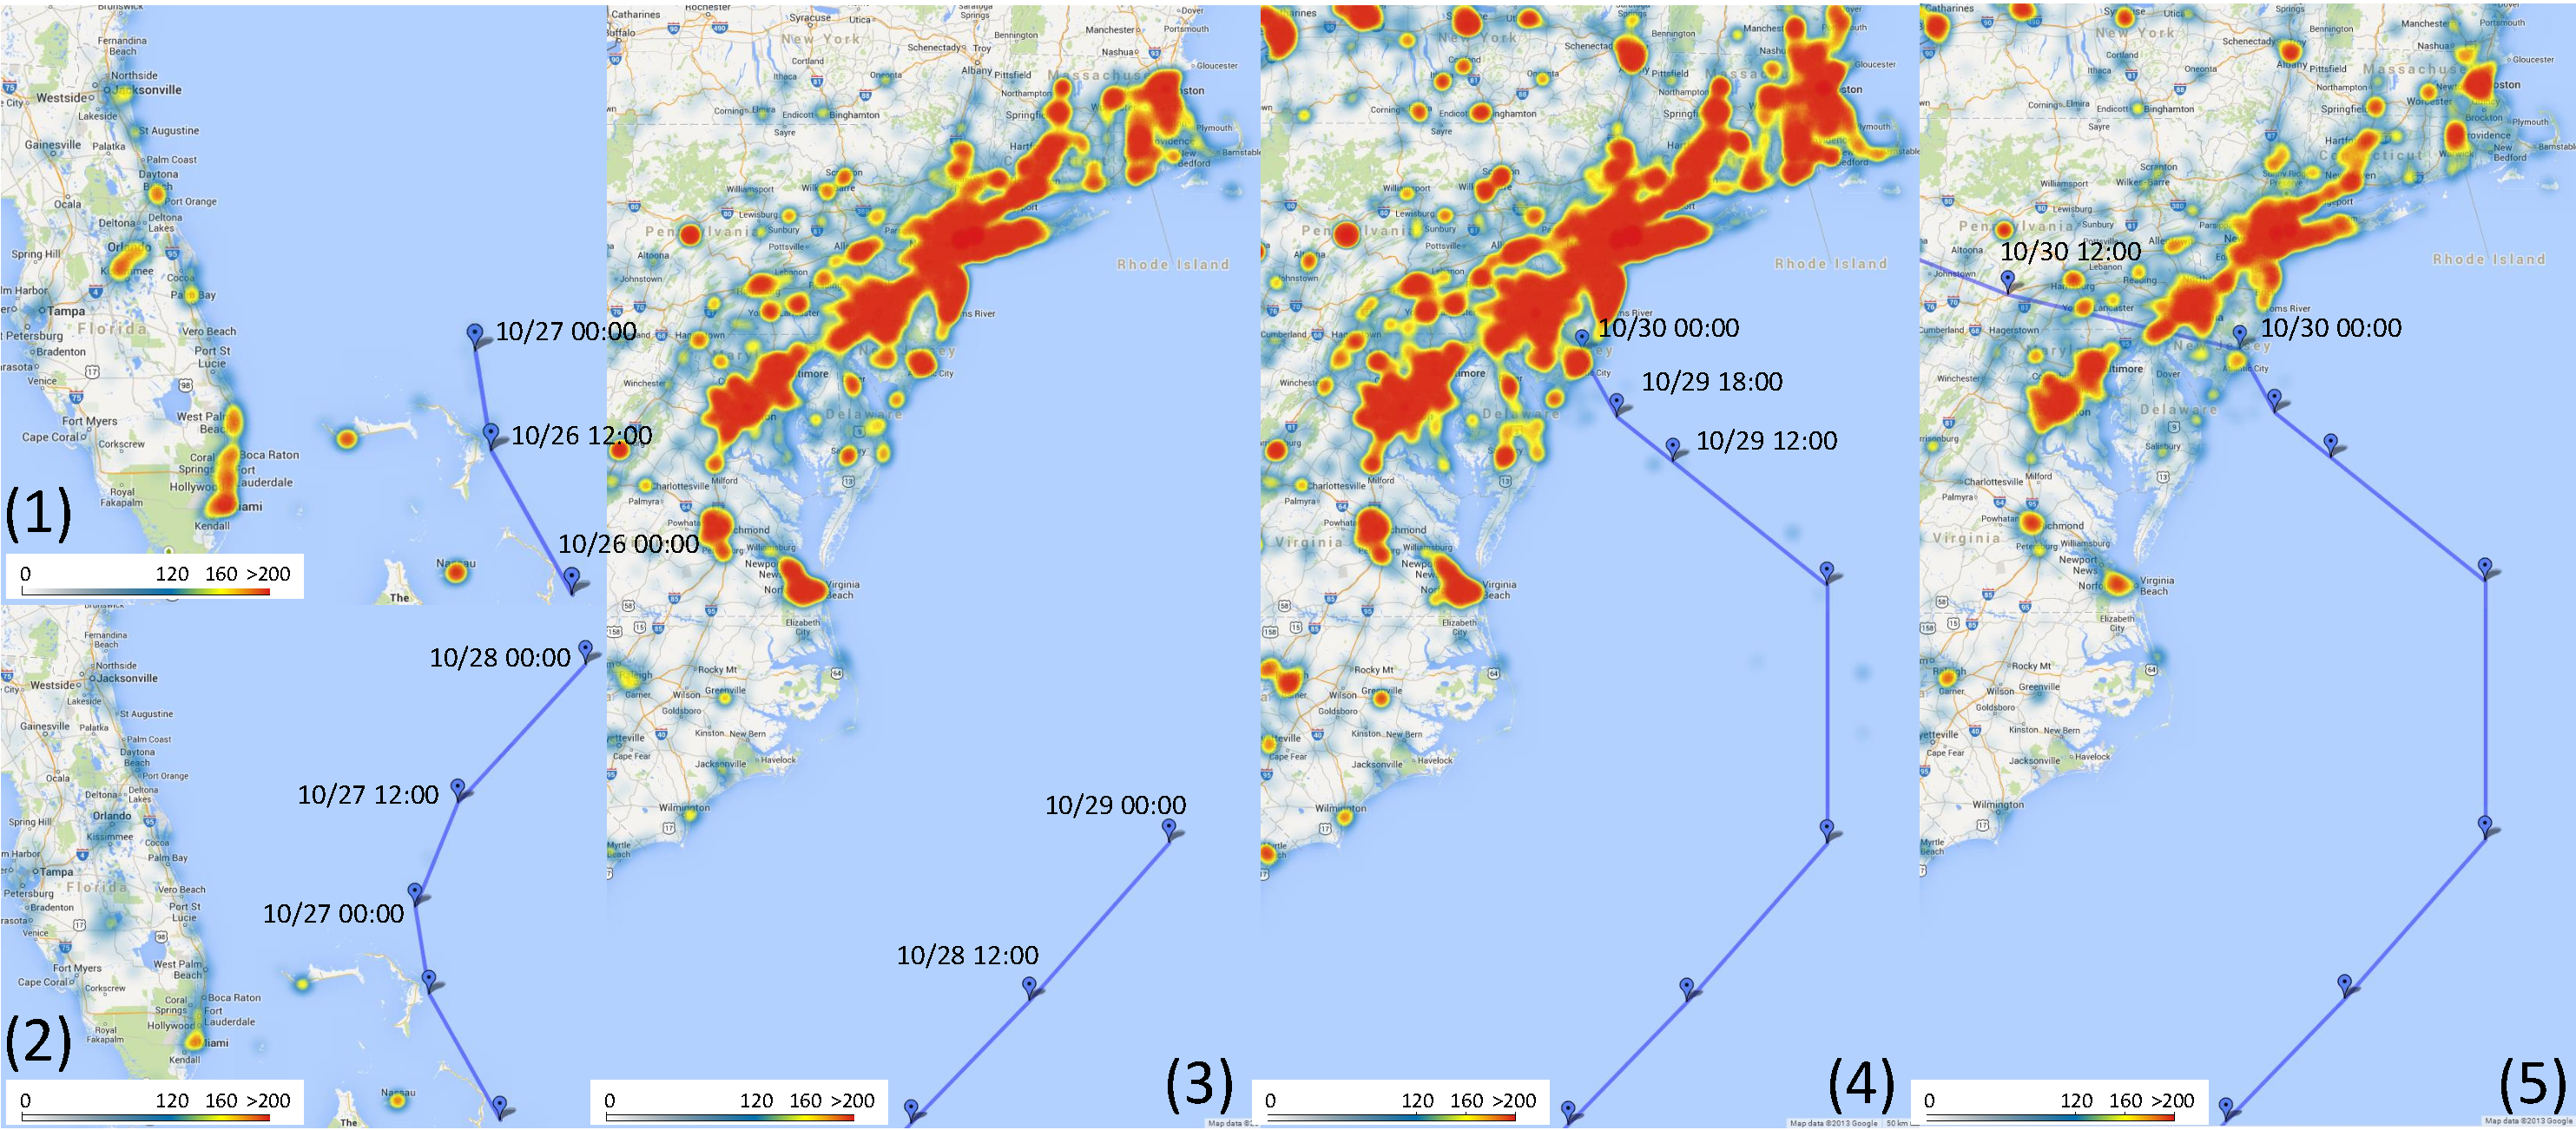
\includegraphics[width=1.0\linewidth]{East_Coast_v7}
\caption{Distribution of Twitter users of each consecutive date (Oct. 26 $\sim$ 30, 2012), who post hurricane related Tweets on the southeastern (1 and 2) and northeastern coast (3, 4, and 5) area of the United States. We can see the variance of Twitter user reactions along the track of the hurricane center locations.}
\label{fig:east_coast}
%\vspace{-0.4cm}
\end{figure}

Twitter users also actively respond to the severe weather conditions.
In Figure~\ref{fig:east_coast}, we indicate that the distribution pattern of Twitter users had dynamically varied along the track of the hurricane center locations.
When Sandy moved to the southeastern coast on October 26th, there were bursts on eastern Florida's coast (Figure~\ref{fig:east_coast}~(1)).
Next day, the bursts disappeared, because Sandy moved towards the northeast away from the east coast of United States (Figure~\ref{fig:east_coast}~(2)).
Sandy kept moving towards a few hundred miles southeast of North Carolina on October 28th (Figure~\ref{fig:east_coast}~(3)).
In the next day, the hurricane's track bent towards the north and the hurricane made landfall at night in the northeast of Atlantic City 
(Figure~\ref{fig:east_coast}~(4)).
Throughout the days, Twitter users were actively reacting to Hurricane Sandy' arrival in a wide range of areas.
After the landfall, the storm turned toward the northwest and was gradually weakened.
The big outbreaks were diminished on October 30th as shown in Figure~\ref{fig:east_coast}~(5).
As shown in the figures, we can see how Twitter users reacted according to the spatiotemporal pattern of the severe weather conditions in the social media domain.
%The Twitter user distributions along the track of the hurricane helps the users to understand the situations and further analysis.

%\textbf{Damage Area along the Tornado's Path:} 
\textbf{Damage Area from a Tornado:} An extremely strong Tornado passed through the city of Moore in southern metropolitan Oklahoma City~\cite{WKP:2013:MOORE} in the afternoon on May 20th, 2013.
The larger than one-mile-wide tornado damaged the city with a wind speed of more than 200~mph.
Figure~\ref{fig:tornado} shows the damaged part of the city.
The tornado entered the area at about 3:16 PM and exited the area after about 10 minutes.
We visualize the distribution of Twitter users on the map during 24 hours, from May 20th 4:00 PM to 21st 4:00 PM.
%This result represents the situation after the city was severely damaged by the tornado.
We also overlay an approximate extent of tornado damage (transparent orange color) and locations of multiple infrastructures, such as schools, hospitals, and supermarkets, on the map view.
Since the tornado suddenly happened and disappeared, we were not able to find significantly abnormal patterns before and during the event. 
%In Section~\ref{sec:discussion}, we will discuss about this in detail.
After the disaster event, however, many Twitter users moved toward some specific areas: two elementary schools, a medical center, a theater, and two large supermarkets.
The two elementary schools, the medical center, and the theater were located within the highly damaged area and they were severely destroyed.
Also many people were hurt and died in these infrastructures.
The increased number of Twitter users was probably due to the fact that many people went to these places in order to rescue the victims~\cite{TWITCHY:2013:CHG}.
Moreover, people might have gone to supermarkets to obtain indispensable things.
In Figure~\ref{fig:tornado}~(1), the heatmap shows a normal situation of Twitter user distribution in the same area.
The distribution is very different from the situation after the tornado hit the area.
This example demonstrates how our visual analytics system enables the analysts to analyze public responses using spatial disaster data and infrastructure data for disaster management.

\begin{figure}[tbh]
\centering
%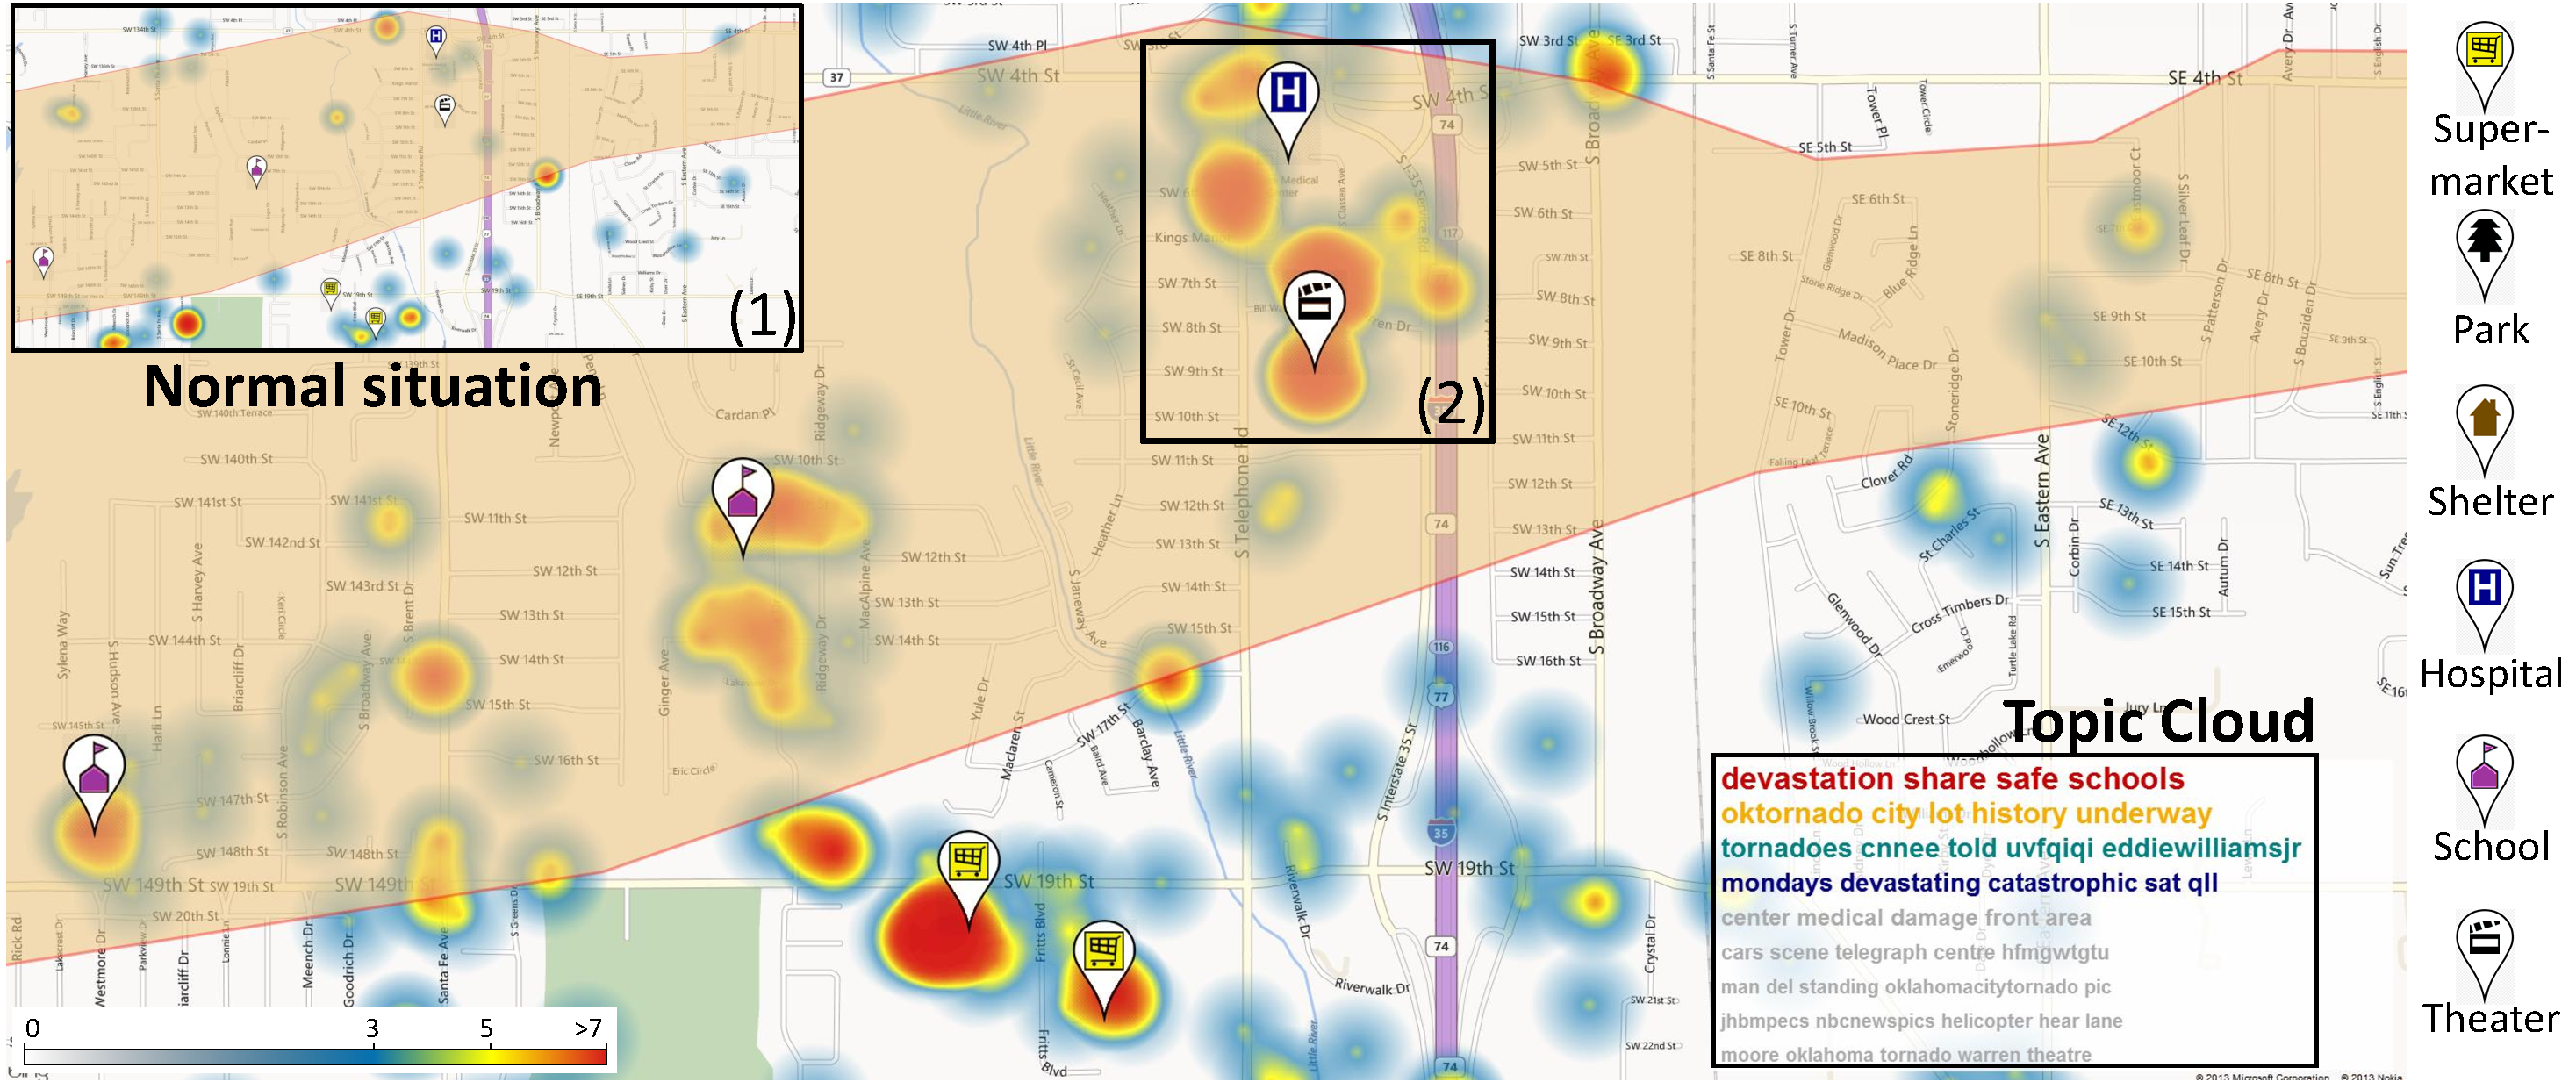
\includegraphics[width=0.9\linewidth]{Tornado_v9}
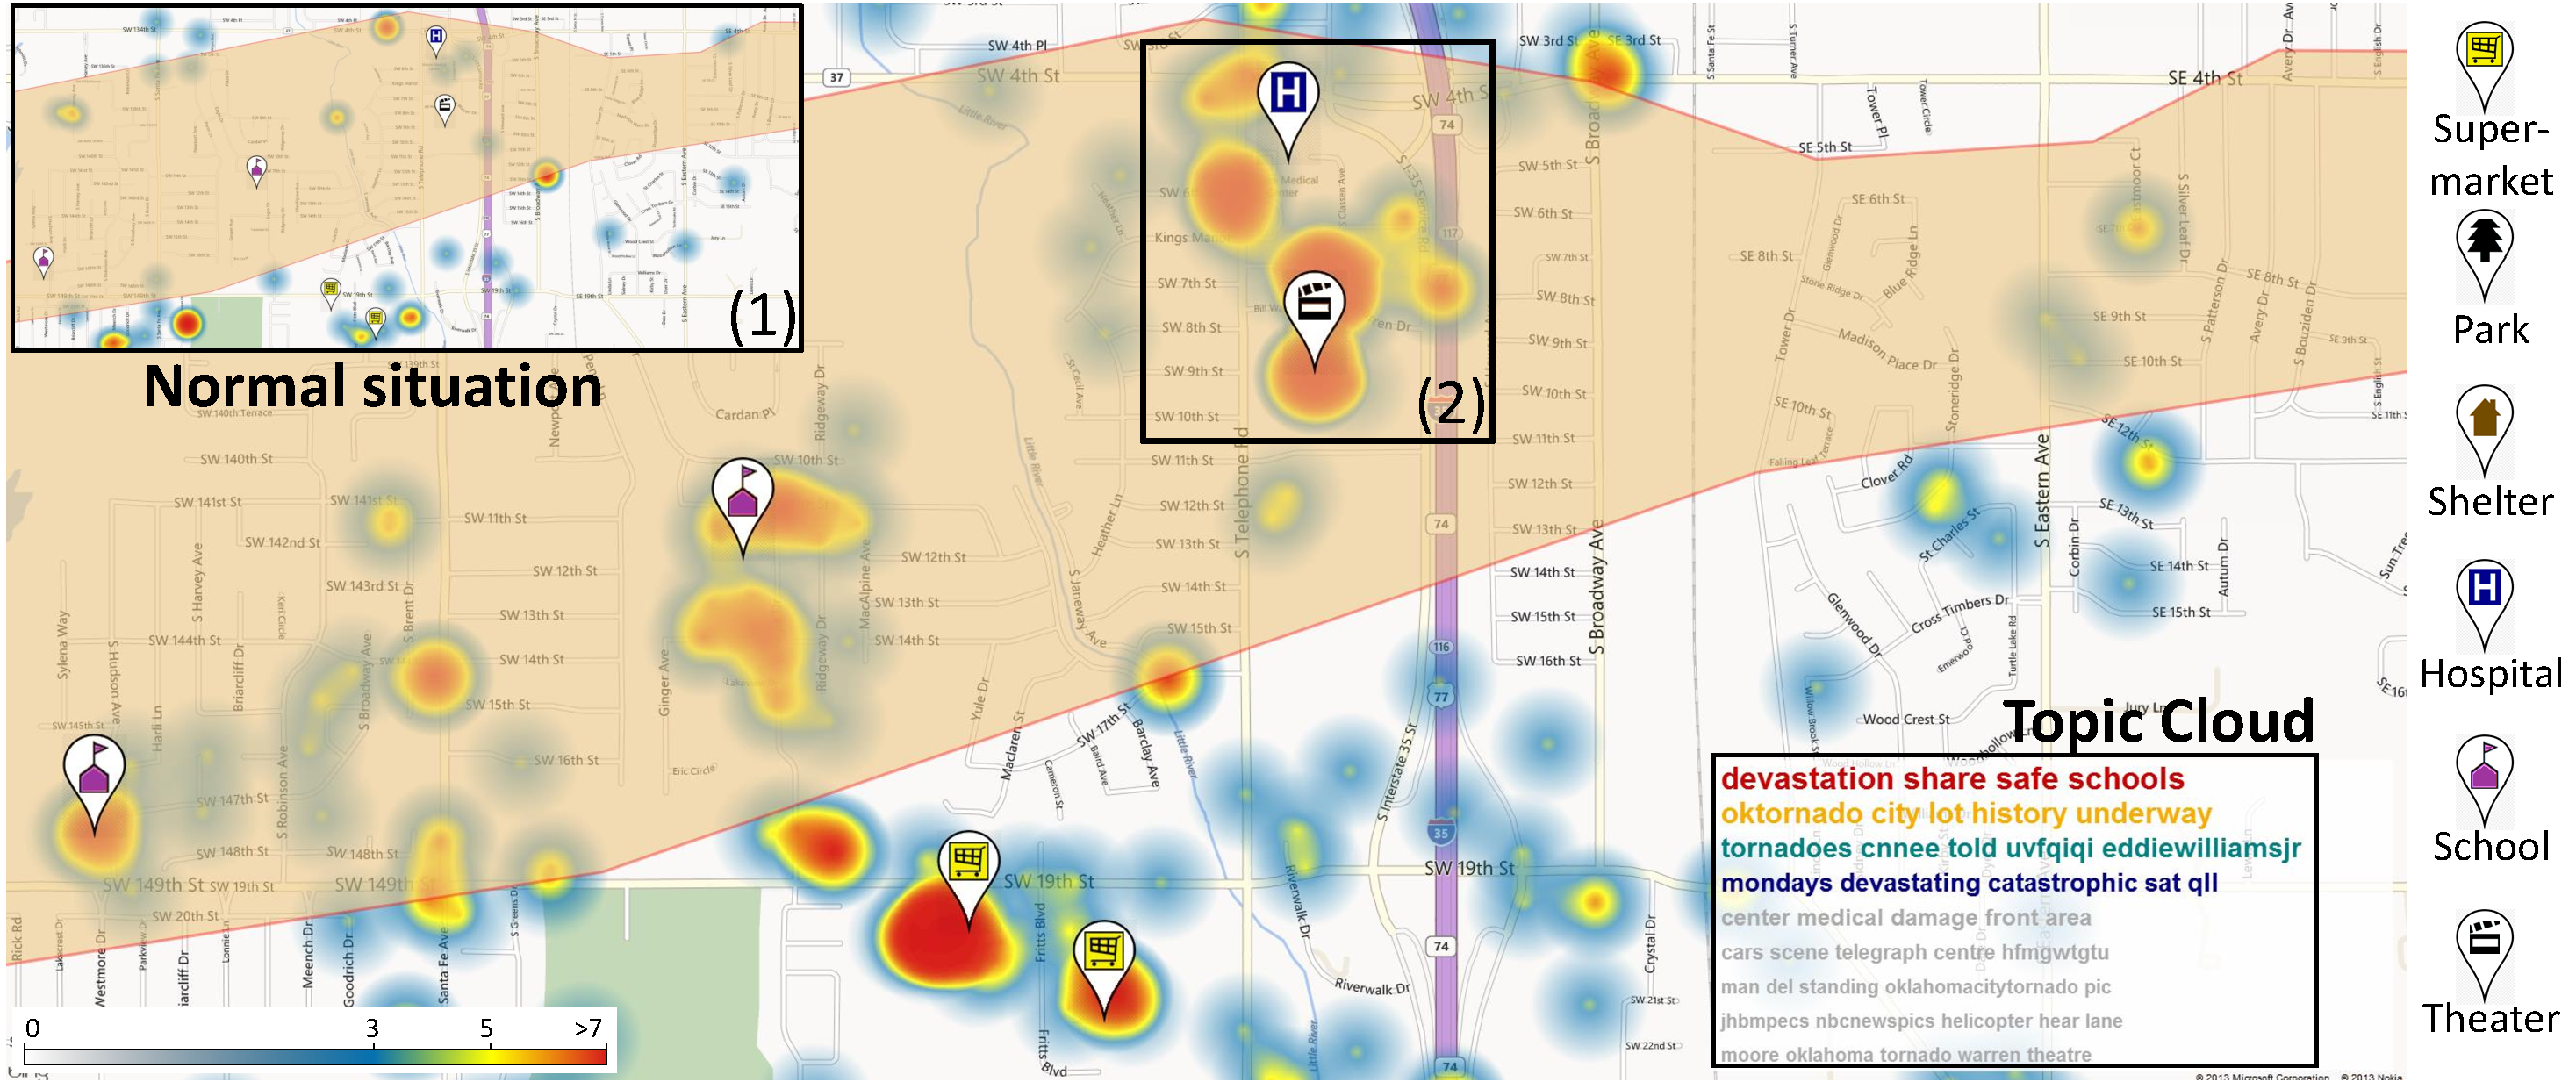
\includegraphics[width=1.0\linewidth]{Tornado_v9}
\caption{Spatial pattern of Twitter users during 24 hours in the city of Moore after damages from a strong tornado. Relatively many people moved to severely damaged areas after the disaster. This situation is much different from the previous normal situation (1). We selected a specific region (2) that includes severely damaged areas in order to extract topics (3) from Tweets within the selected area.}
\label{fig:tornado}
%\vspace{-0.2cm}
\end{figure}

\subsubsection{Abnormal Topic Analysis}
\label{sec:abnormal_topic_analysis}
\begin{figure}[tb]
\centering
%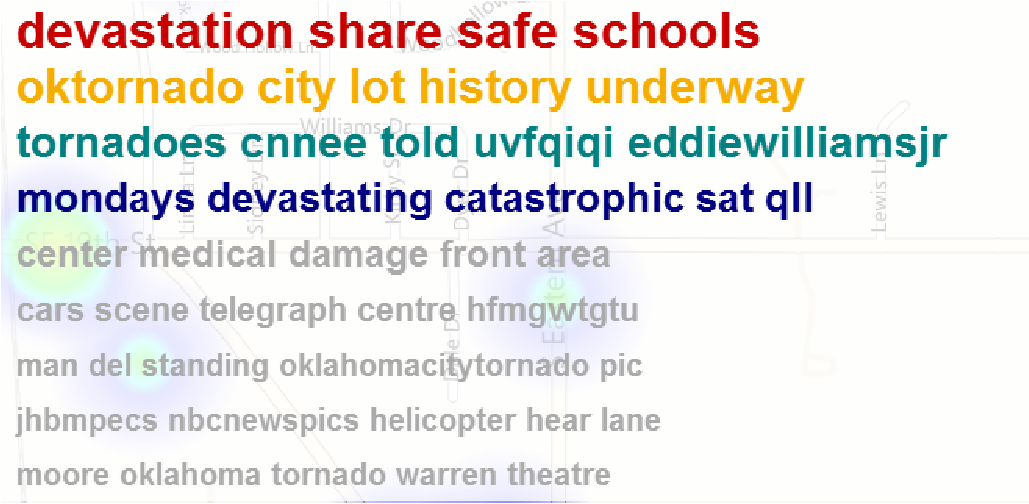
\includegraphics[width=0.85\columnwidth]{Topiccloud_v2}
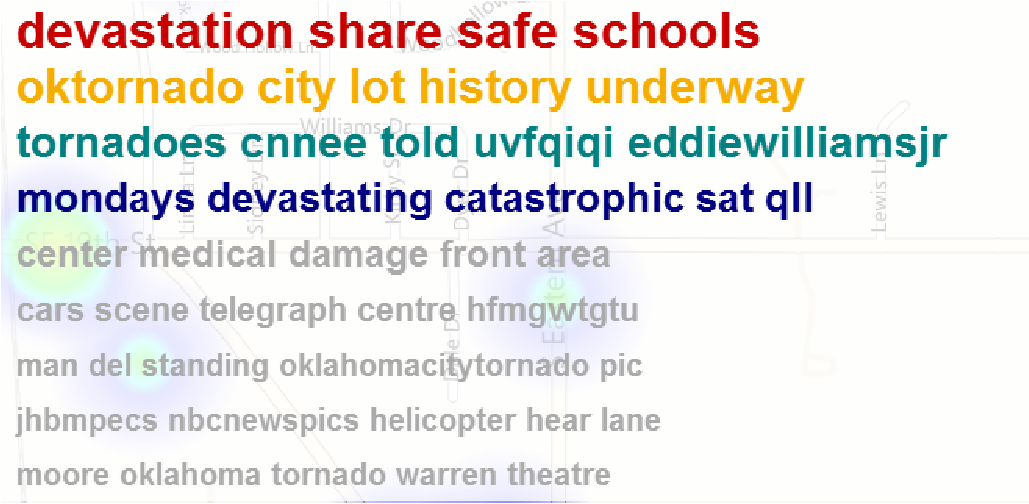
\includegraphics[width=0.8\linewidth]{Topiccloud_v2}
\caption{Topic cloud: Topics from Tweets within the selected area in Figure~\ref{fig:tornado}~(2) are ordered by their abnormality scores.}
\label{fig:topic_cloud}
%\vspace{-0.4cm}
\end{figure}

Our system also provides analysts with abnormal topic examination within the microblog data.
Each Twitter message provides not only spatiotemporal properties, but also textual contents.
The text messages are also important to understand and examine the emergent situations.
Our system allows the analysts to extract major topics from many Tweets posted within a specific area using the LDA~\cite{Blei:2003:LDA}.
We also employ, then, the STL~\cite{Cleveland:1990:SAS} to identify unusual topics within the selected area.
For each extracted topic of the LDA topic modeling, our algorithm retrieves messages associated with the topic and then generates a time series consisting of daily message counts from their timestamps.
The time series can be considered as the sum of three components: a trend component, a seasonal component, and a remainder.
Under normal conditions, the remainder will be identically distributed Gaussian white noise, while a large value of the remainder indicates substantial variation in the time series.
Thus, we can utilize the remainder values to implement control chart methods detecting anomalous outliers within the topic time series.
We have chosen to utilize a seven day moving average of the remainder values to calculate the z-scores.
Note that we use the z-score as the abnormality score in this work.
If the z-score is higher than 2, events can be considered as abnormal within a 95\% confidence interval.
The details of these techniques are described in the previous work~\cite{CHAE:2012:SSM}.
We select a sub area in Figure~\ref{fig:tornado}~(2) that includes severely damaged areas: the selected region (black rectangle) on the map.
The extracted topics, which are ordered based on their abnormalities, are displayed as Topic Clouds at the bottom-right corner (Figure~\ref{fig:tornado}~(3)) on the map.
The topic cloud is enlarged and shown in Figure~\ref{fig:topic_cloud}.
In this case study, most topics are related to the disaster event. 
However, the last topic\textemdash \textit{moore, oklahoma, tornado, warren, theatre}, has a relatively low abnormality although they seem related to the disaster event, because tornadoes frequently occur in the area.
%Our abnormal topic analysis enables the analysts to understand what situations are going within the area.
Figure~\ref{fig:abnormality_graph} shows an abnormality graph for the first topic in Figure~\ref{fig:topic_cloud}.
The abnormality score for the topic had significantly increased when the tornado hit the region on May
20th (Marked region). As shown in Figure~\ref{fig:abnormality_graph}, the abnormality score (6.75) is much higher than the average abnormality score(0.42); therefore, the analysis of the microblog data provides a statistically significant difference during this severe weather condition.



\begin{figure}[tb]
\centering
%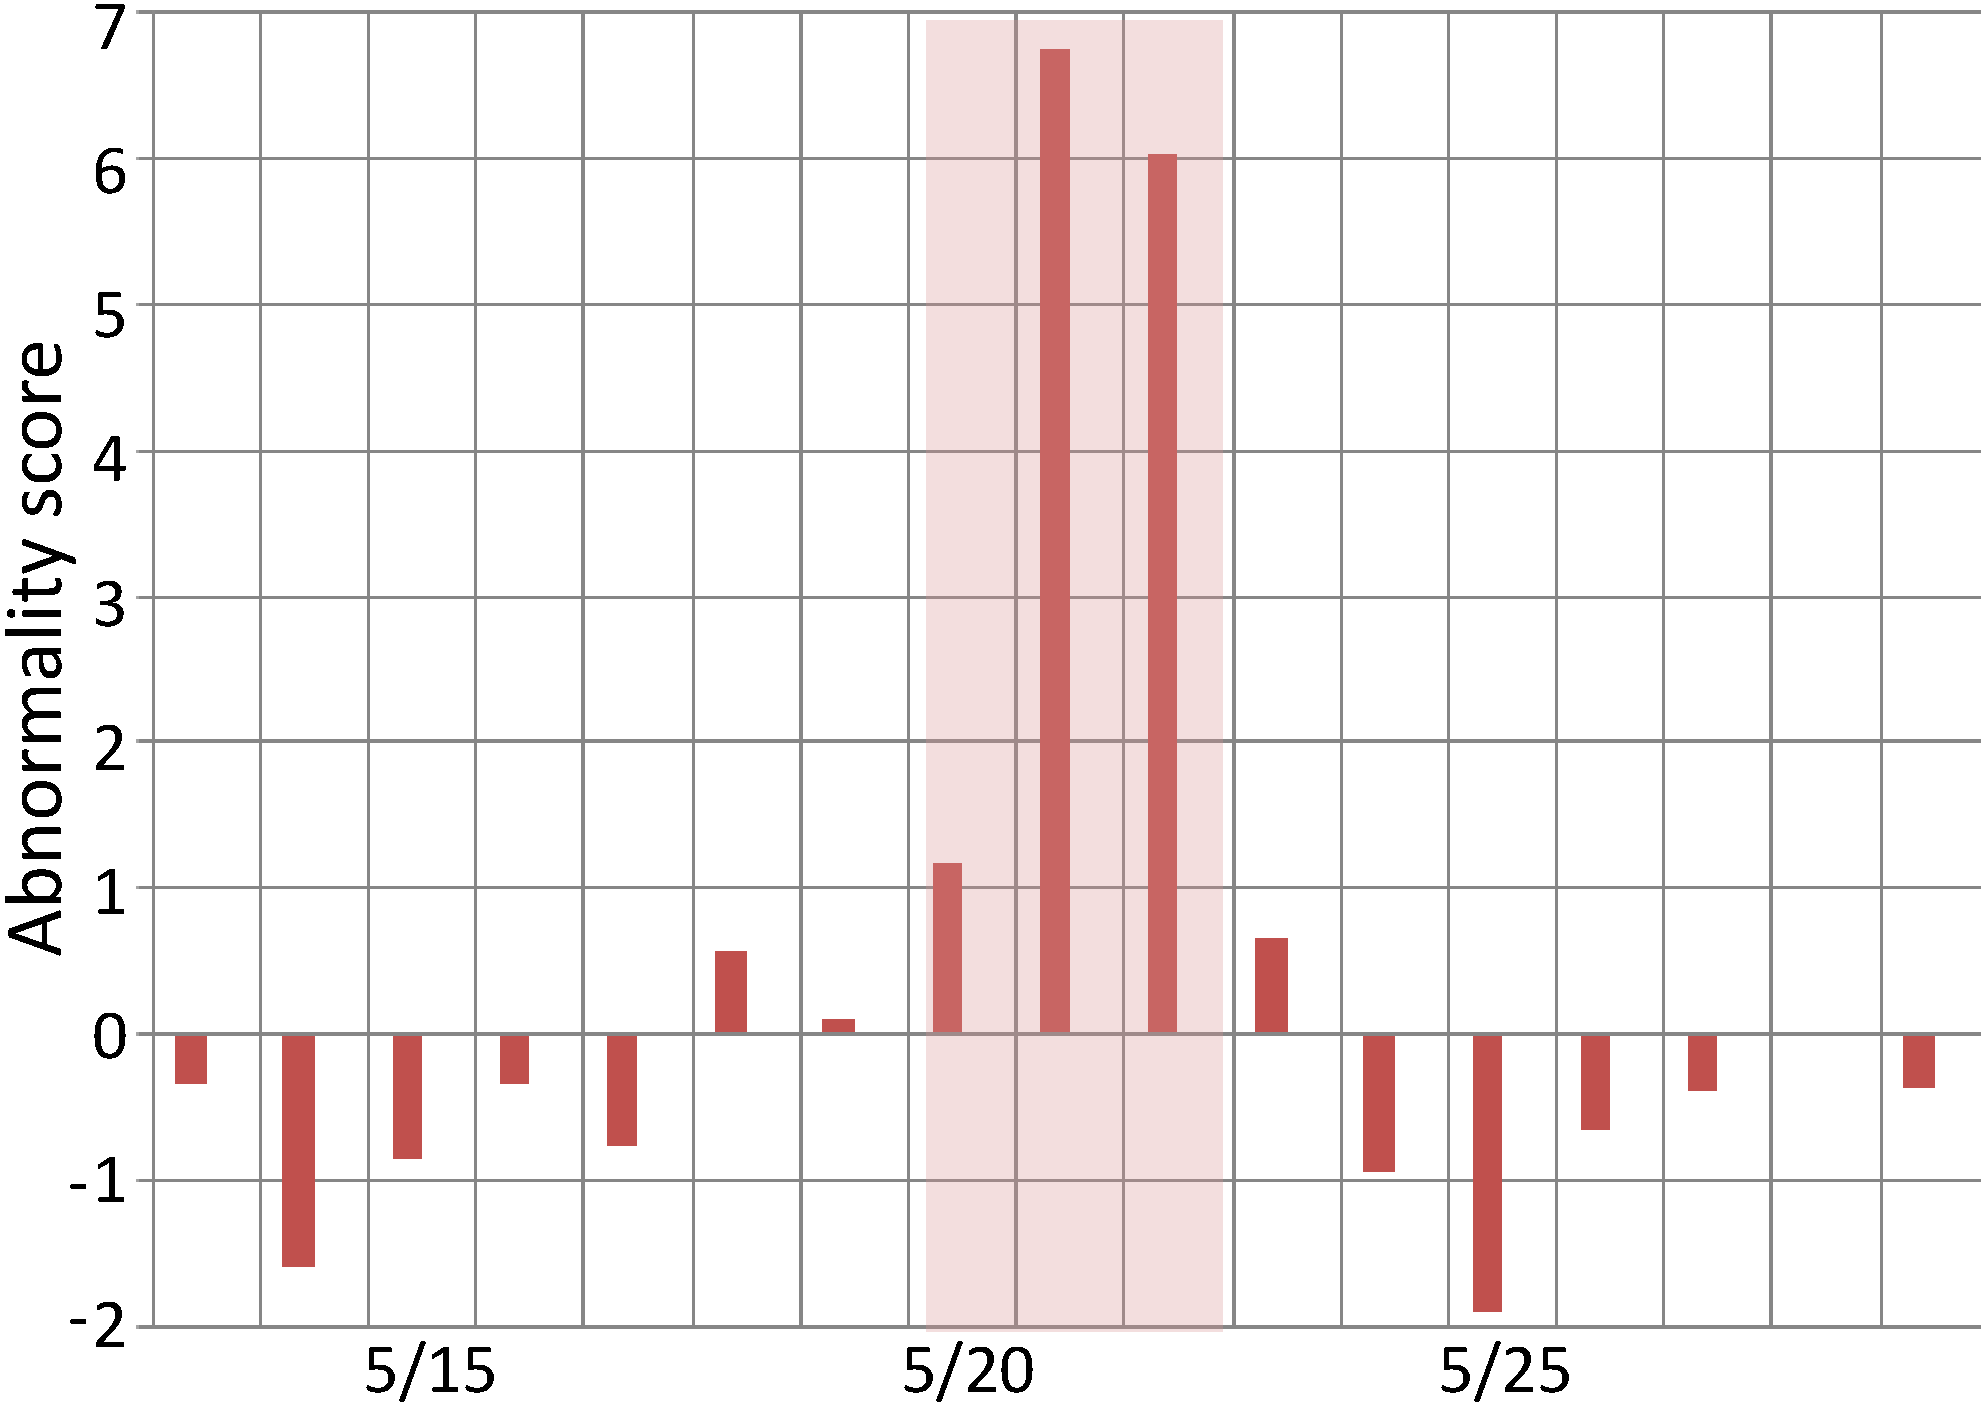
\includegraphics[width=0.7\columnwidth]{Topiccloud_zscore_graph_v3}
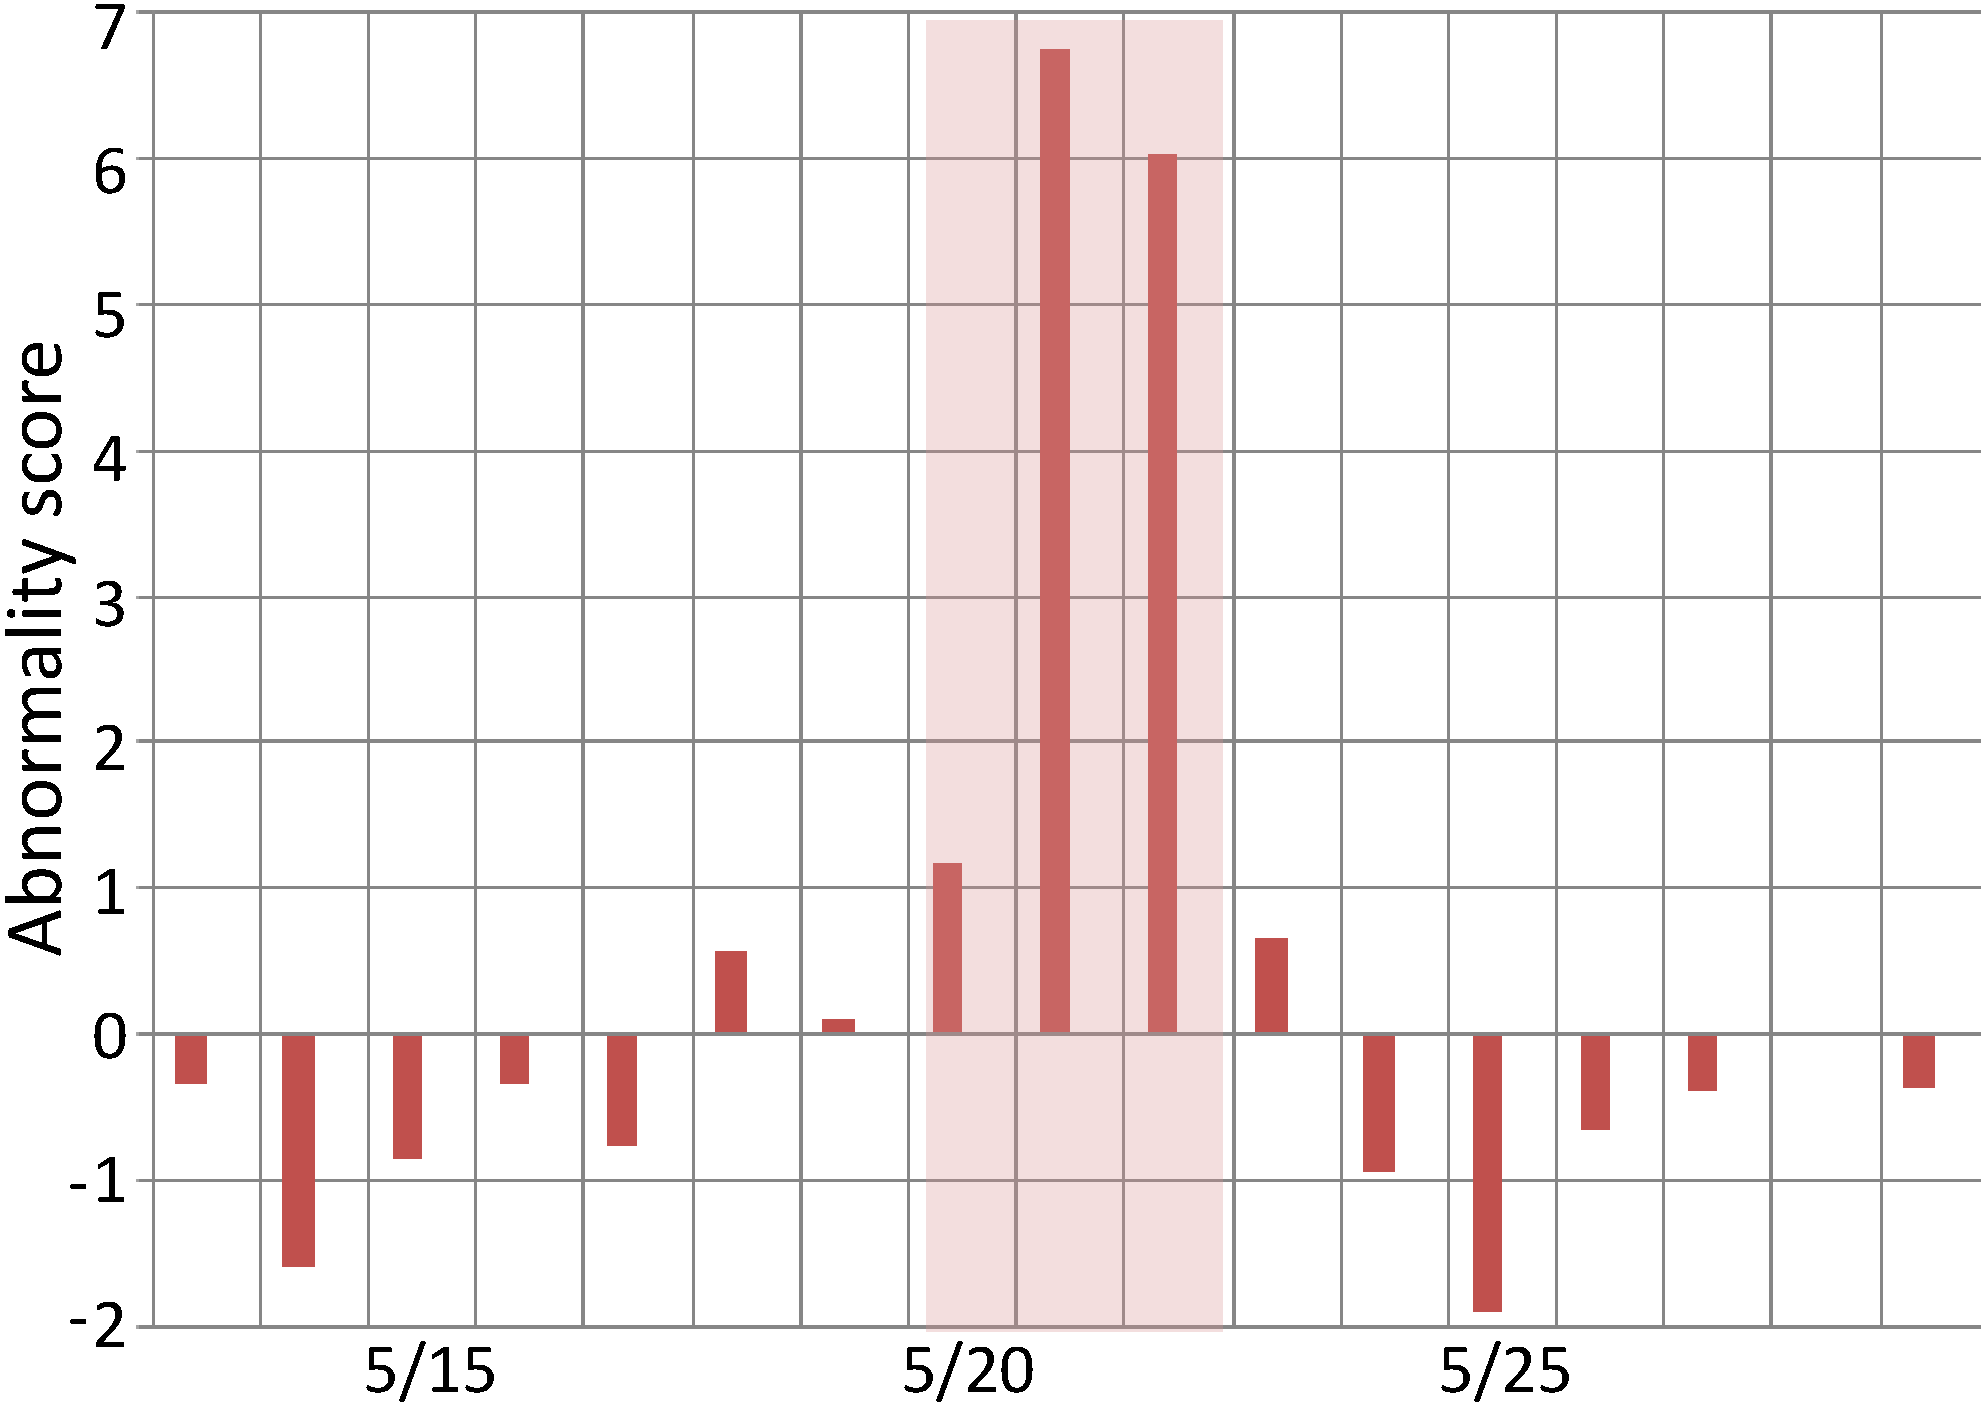
\includegraphics[width=0.8\linewidth]{Topiccloud_zscore_graph_v3}
\caption{Abnormality of the first topic in Figure~\ref{fig:topic_cloud}. 
The abnormality score of the topic had significantly increased when the tornado hit the region on May 20th (Marked region).}
\label{fig:abnormality_graph}
%\vspace{-0.4cm}
\end{figure}


\subsection{Temporal Pattern Analysis}
\label{sec:temporal_pattern}
%
%Describe the graph
%In Section~\ref{sec:spatial_analysis}, we present spatial analysis of social media and spatial decision support using multiple types of supplementary data in order to reveal where and why a number of people move.
In the previous sections, we presented the spatial analysis of social media and spatial decision support. 
In this section, we demonstrate analysis of the relationships between the temporal patterns of the number of Twitter users and certain public situational behaviors:
%using time-stamp information of Tweets
how many people go where and how different is it from previous situations?
Analysis of temporal trends and relationships between data values across space and time provides underlying insights and improves situational awareness~\cite{Maciejewski:2010:FHP, Malik:2011:DTC}.


After selecting the initial spatiotemporal context of Tweets as a basis for the analysis, the analysts can explore the temporal patterns of the number of Twitter users who posted Tweets within the spatial boundary using the bar chart as shown in Figure~\ref{fig:graph}.
The values of each bar are the number of users in four hour intervals and represent data two weeks before and after the selected date.
Once a mouse cursor hovers over one of the bars in the graph, every bar that corresponds to that time period, is highlighted in dark yellow color as shown in Figure~\ref{fig:graph}.
As previously mentioned, the heatmap in the figure shows the Twitter user density distribution from 12:00 PM to 4:00 PM on October 28th, right after the announcement of the evacuation order.
We select a hotspot that includes one of the supermarket locations: the selected region (black rectangle) on the map in Figure~\ref{fig:heatmap_manhattan} (Right).
We can indicate that the number of Twitter users (red rectangle in Figure~\ref{fig:graph}) in the corresponding time period is higher than for the same time period from other dates (October 14th, 21st and November 4th, 5th) by 35\% more from the average.
Moreover, there is another interesting finding\textemdash the number of people during each of the following time frame (4:00 $\sim$ 8:00 PM) on the dates from the previous weeks are higher than the number of people in the selected time frame.
This is because many shoppers were lining up at stores and emptied the shelves to prepare for Hurricane Sandy.
Some actual Twitter messages posted in the area are following: \textit{\textquoteleft The line at Trader Joes is unbelievable ...\textquoteright} and \textit{\textquoteleft There is amazing line here ...\textquoteright}.
Furthermore, since October 29th, the number of people has significantly decreased because most residents left the area before the arrival of the hurricane.
The increase in the number of people after one week reflects that some people came back to the area.
% and even shows when the stores reopened.

%Social media use rises during disasters as people seek immediate and in-depth information%~\cite{STAR}.
%reflect that the number users increased during sandy, but the situation had been gone since evacuation or severe damage for example, power outage caused by flooding and strong wind.

\begin{figure}[tbh]
\centering
%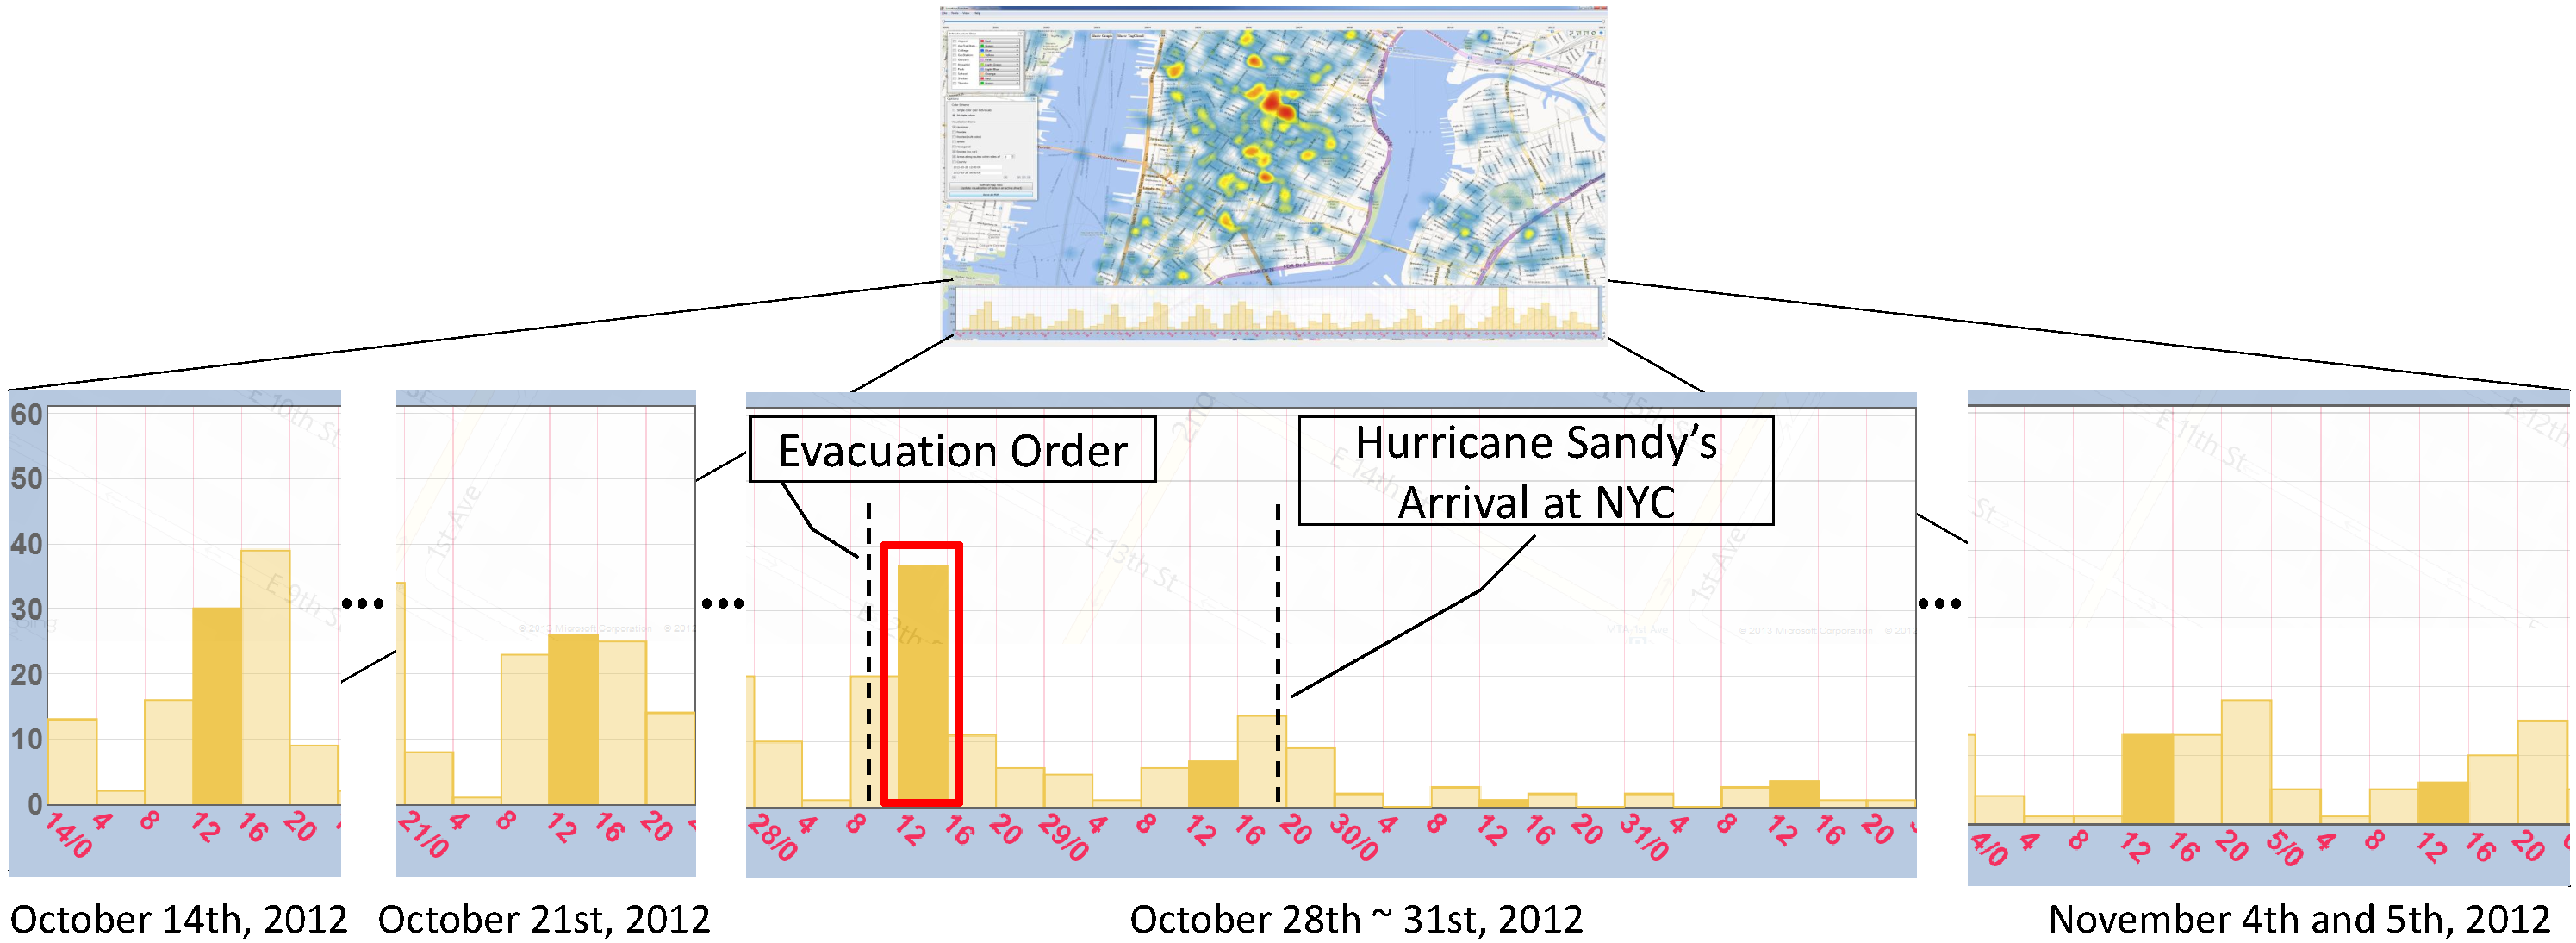
\includegraphics[width=0.80\linewidth]{graph_system_v4}
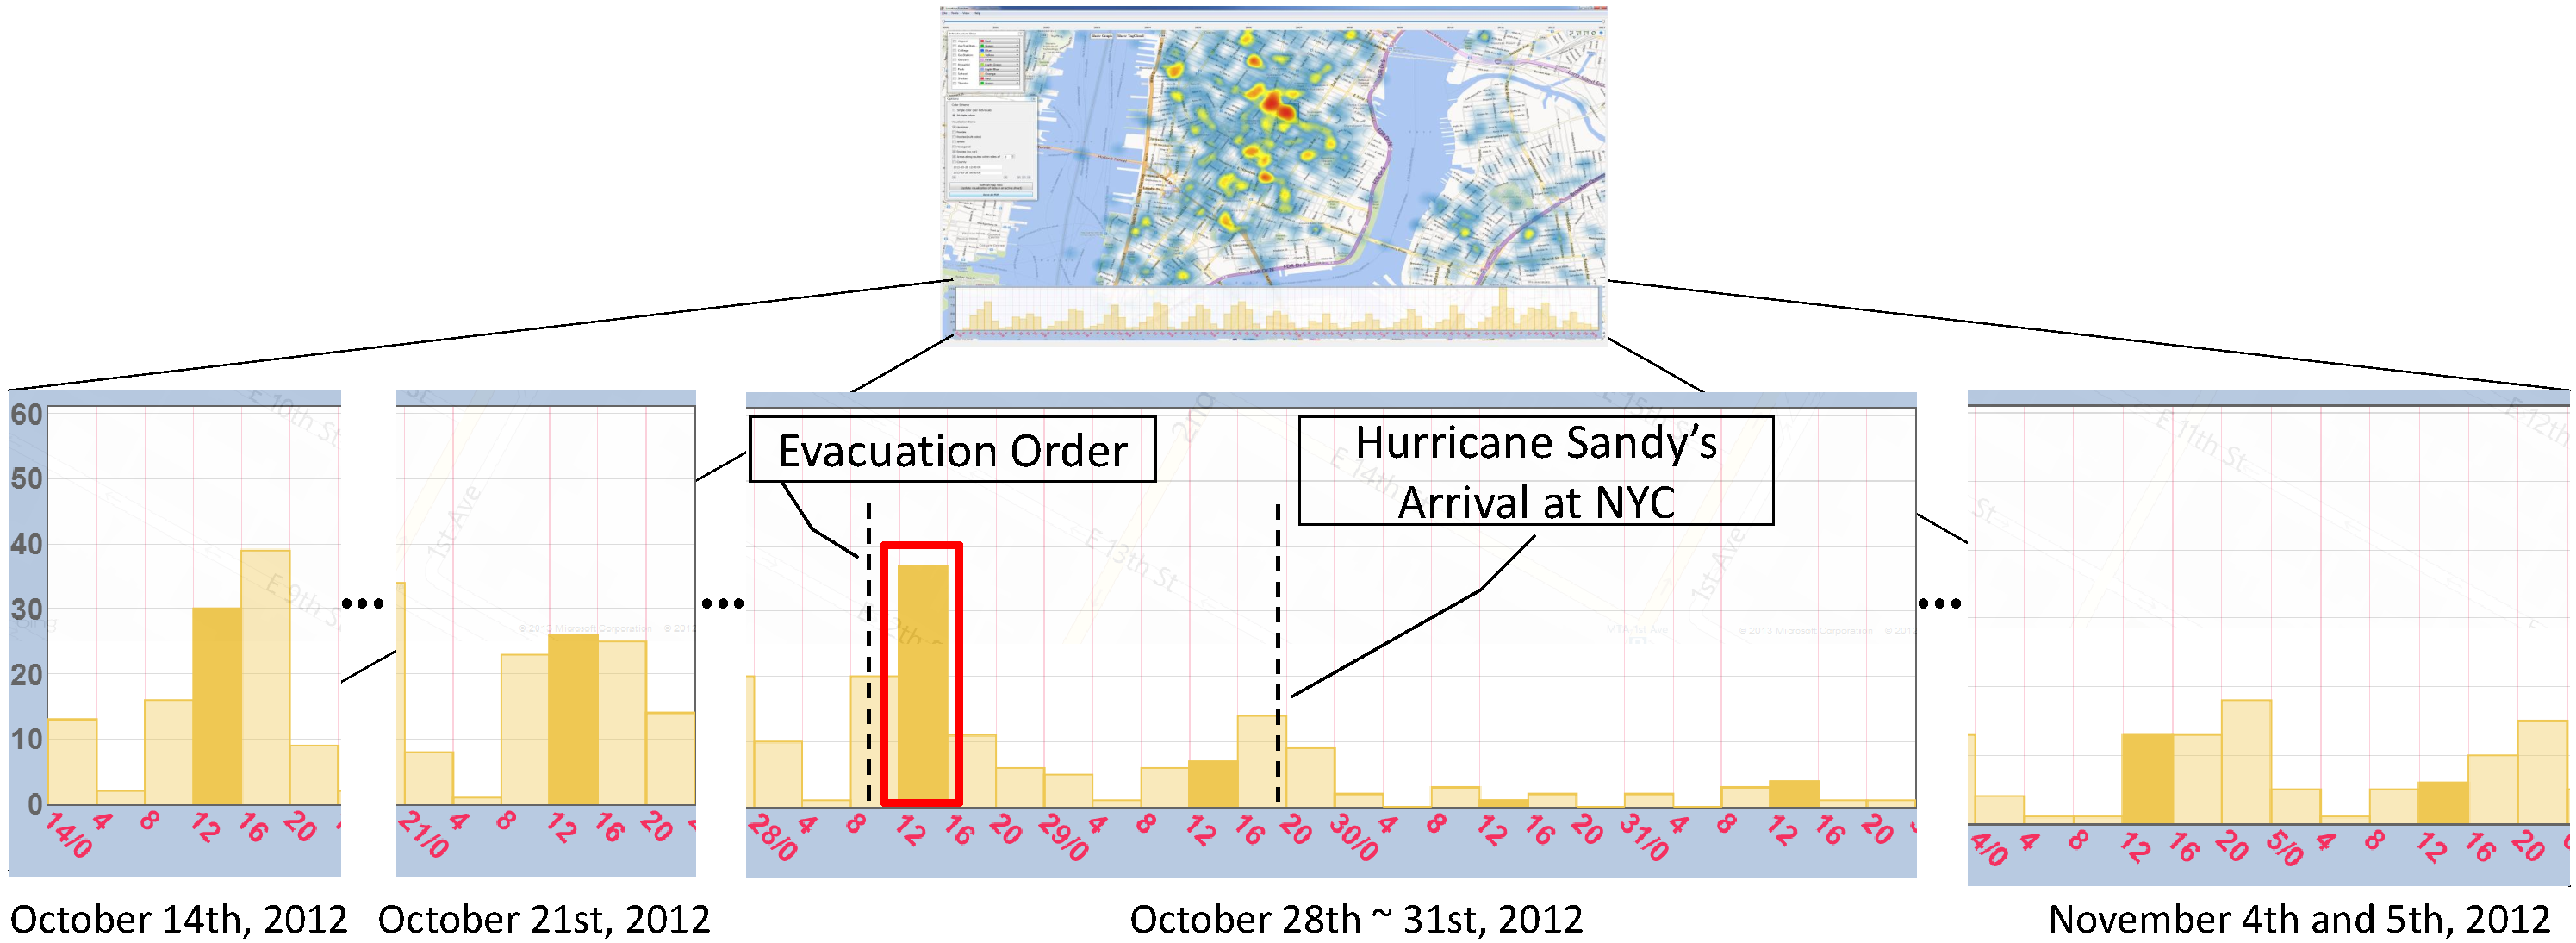
\includegraphics[width=1.0\linewidth]{graph_system_v4}
\caption{Temporal analysis for public behaviors during the disaster event, Sandy. Top shows our entire system view. 
The bar chart (Bottom) for the number of Twitter users within the selected region including a supermarket in Figure~\ref{fig:heatmap_manhattan} (Right) in four hour intervals is shown.
%some interesting time frames of the entire plot on the system. 
We see that many people went to the supermarket right after the evacuation order.}
\label{fig:graph}
%\vspace{-0.4cm}
\end{figure}





\subsection{Spatiotemporal Visualization}
\label{sec:spatiotemporal_visualization}

\begin{figure}[tb]
\centering
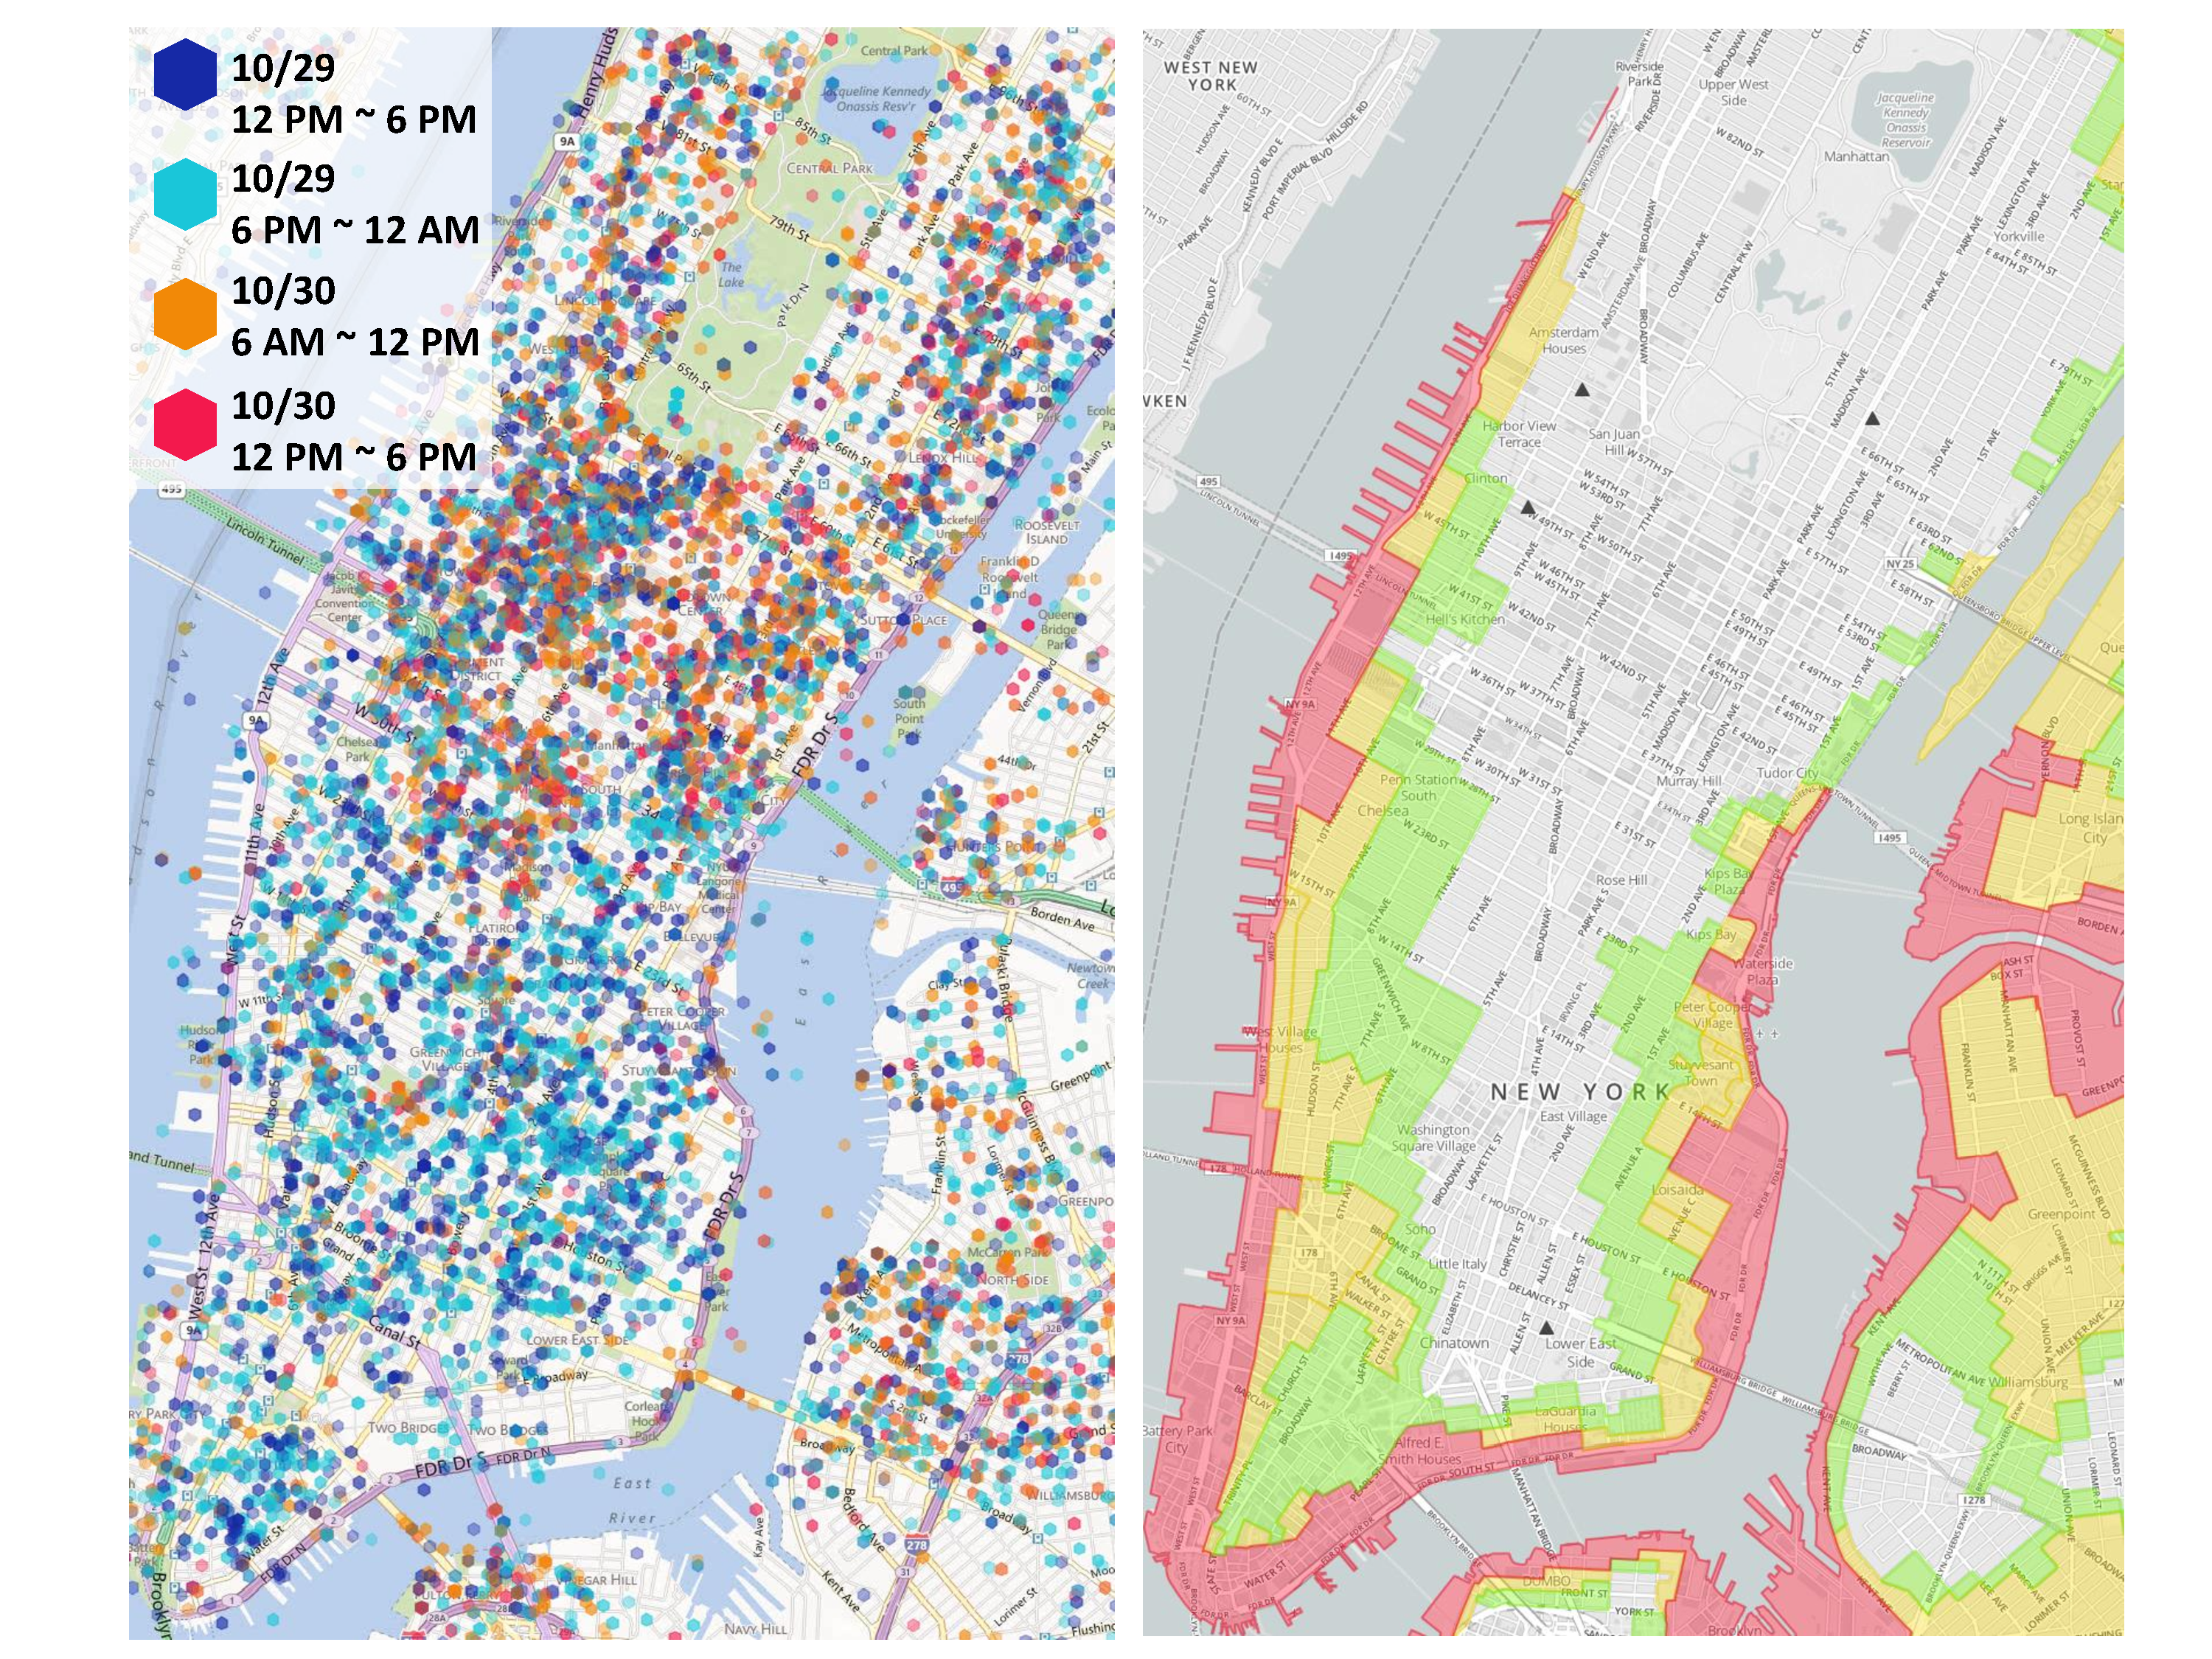
\includegraphics[width=1.0\linewidth]{spatiotemporal4}
\caption{Visualization for spatiotemporal social media data (Left).
A hexagon represents the spatial (position) and temporal (color) information of a Tweet.
Hurricane evacuation map~\cite{NYC:2012:HEM} (Right). Residents in Zone A (red) faced the highest risk of flooding, Zone B (yellow) and Zone C (green) are moderate and low respectively.}
\label{fig:spatiotemporal}
%\vspace{-0.8cm}
\end{figure}


There is abundant research published on the topic of spatiotemporal data visualization.
Still, exploration of time-referenced geographic data is still a challenging issue~\cite{Andrienko:2003:ESV}.
We introduce a modest visualization that enables analysts to analyze both aspects: space and time in a single view.
Each Tweet is independent and contains multiple properties, such as location, time, the number of re-Tweet, etc.
In this study, therefore, we utilize a glyph-based visualization to depict both location and time aspects of the independent data record using two visual features.
As shown in Figure~\ref{fig:spatiotemporal}~(Left), each hexagon corresponding to a Tweet represents the spatial and temporal information where the center of each hexagon is the location of each Tweet and the color represents its posting time.
In other words, space and time properties are encoded in a single visualization to harness the spatial analysis features of human visual perception~\cite{Treisman:1980:FIT}.
In Figure~\ref{fig:spatiotemporal}~(Left), the hexagons with blue~(12 PM $\sim$ 6 PM) or green~(6 PM $\sim$ 12 AM) ) color correspond to Tweets published on October 29th, 2012 and ones with orange or red color correspond to Tweets posted on the following day after the hurricane.
New York City announced the evacuation of Zone~A~(red color) in Figure~\ref{fig:spatiotemporal}~(Right); residents in Zone~A faced the highest risk of flooding, whereas, Zone~B~(yellow color) and Zone~C~(green color) are moderate and low respectively.
In the visual representation, analysts can indicate overall spatiotemporal patterns of people and their movements during the disaster event\textemdash many people still remained at home one day after the mandatory evacuation order, but most people left home on the following day as the hurricane damaged the city.
%\vspace{-0.3cm}

\section{Discussion and Evaluation}
\label{sec:discussion}
%
In this work we found out that the public responses to disaster events in social media streams are different according to the disaster event types.
Hurricane Sandy had a long time duration\textemdash more than one week, and affected a wide range of areas.
Therefore, there were many reactions in the potential damage area before the hurricane impacted the area.
%We could also indicate some hotspots in the area during the event.
However, no or significantly less hotspots were found right after the hurricane passed over the area.
This was because the hurricane severely affected the areas\textemdash communication facility damage and power outages occurred in the area.
Moreover, we found out that unusual post-event situations in the Twitter user distribution continued for a certain time period from a couple of days to more than one week as shown in Figure~\ref{fig:east_coast} and~\ref{fig:graph}.
%~\ref{fig:atlantic_coast}.
The analysts could estimate how long it took for the reconstructions in the areas.
%Hurricane-force winds can extend outward to about from 25 miles to more than 300 miles from its center.

Regarding the tornado case, we intended to find abnormal patterns in the Twitter user distribution before and during the disaster event
but there was no unusual patterns in the area.
In contrast to the hurricane, the tornado generally affected the areas relatively shortly, for example, a few minutes to an hour.
The abrupt natural disaster did not strongly influence the social media stream before and even during the event.
However, as shown in Figure~\ref{fig:tornado}, we were able to find many hotspots within the damaged areas after the tornado passed.
In fact, the tornado damaged some small areas (i.e., a couple of miles wide), in contrast to the wide range of damaged areas for the hurricane case.
This indicated that communication facilities were still available and many people were interested in the disaster, similar to the hurricane.
Thus, our social media analysis could support the analysts to make plans and manage for the emergent situations according to the types of the disasters.
%The number of Tweets are very different between rural and urban areas.

The above cases demonstrate how our system supports spatial decision making through evaluation of varying-density population area to determine changes in behavior, movement, and increase overall situational assessment. This increased spatial activity and behavioral understanding provides rapid situational assessment and provides insight into evolving situational needs to provide appropriate resource allocation and other courses of action (e.g., traffic rerouting, crowd control).

%There is a use case scenario of disaster management support utilizing our visual analytics system.
%Analysts can locate the high density population spots and understand the local situations using our system before or during a disaster event. 
%Then, they can quickly and appropriately respond, such as traffic control to the situations or resource allocation in order to mitigate potential risks.
We requested informal feedback for the usability of our system from users within our universities, and received useful and positive comments and suggestions.
They were interested in the findings of the abnormal situations during the disaster events in Section~\ref{sec:spatial_analysis} and~\ref{sec:temporal_pattern}. They also noted that the use of the infrastructure symbols on the heatmaps improved the legibility of the Twitter user distributions in Figure~\ref{fig:heatmap_manhattan}
and they suggested a visualization for the deviations between multiple heatmaps in order to show the differences clearly, which we plan to develop in the future.
%Furthermore, we are planning to conduct a formal experiment for user evaluation for our system in the future.
%Our system provides a testbed for evaluating the impact of interactive spatiotemporal visual analytics using social media data in disaster management.
%Furthermore, we are planning to conduct a formal user evaluation for 
%the impact of interactive spatiotemporal visual analytics using social media data on disaster management.
%We plan to evaluate: (1) the effect of geospatial visual support to explore and examine public spatial distribution using microblog data; (2) the effect of supplementary spatial information support for spatial decision-making (vs. without any supplementary information); (3) the usability of the glyph-based spatiotemporal visualization; and (4) the performance of the system under different locations, different types of disasters, and different location-based social media data.

%\begin{itemize}
%\item the effect of having geospatial visual support for exploring and examining public spatial distribution using microblog data;
%\item the effect of supplementary spatial information support for spatial decision-making (vs. without any supplementary information);
%\item the usability of the glyph-based spatiotemporal visualization;
%\item and the performance of the system under different locations, different types of disasters, and different location-based social media data.
%\end{itemize}


\section{Summary}
\label{sec:conclusions}
%
In this work we presented a visual analytics system for public behavior analysis and response planning in disaster events using social media data.
We proposed multiple visualizations of spatiotemporal analysis for disaster management and evacuation planning.
For the spatial decision support, we demonstrated an analytical scheme by combining multiple spatial data sources.
Our temporal analysis enables analysts to verify and examine abnormal situations.
Moreover, we demonstrated an integrated visualization that allows spatial and temporal aspects within a single view.
We have still some limitations with these techniques including the potential occlusion issues in the spatiotemporal visualization.
%For future work, we will investigate the flow of public movement before and after disasters and the analysis for recovering from disasters and crises. We also plan to design the glyphs with varied sizes adapting to the zoom level in the spatiotemporal visualization. 
%In addition, 
%%we will conduct a user evaluation of our system in the future.
%we will conduct a user evaluation for the usability and effectiveness of the geospatial visual support,
%and the impact of interactive spatiotemporal visual analytics using social media data on disaster management.
%, the effect of supplementary spatial information support for spatial decision-making (vs. without any supplementary information); (3) the usability of the glyph-based spatiotemporal visualization; and (4) the performance of the system under different locations, different types of disasters, and different location-based social media data.


%This system provides a heat map of people who posted geo-located Tweets around the Manhattan area during specific time periods and allows us to analyze their spatial distribution.
%Our bar chart visualization enables users to analyze the temporal distribution of the number of people tweeting in a given location and time.
%Finally, we provide a visualization that allows users to simultaneously analyze both aspects: space and time using a single view.

%The remainder of this document is structured as follows: 
%Section~\ref{sec:relatedwork} is a review of related work.
%We demonstrate how to improve investigations and analysis for public behavior response to the disaster by spatiotemporal analysis of social media in Section~\ref{sec:body}.
%Finally, we present a conclusion and future work in Section~\ref{sec:conclusions}.

%\subsection{Data and Event}
%\label{sec:data}
%
%\begin{figure}[tb]
%\centering
%\includegraphics[width=0.9\columnwidth]{Sandy_Track}
%\caption{Track of Sandy}
%\label{fig:sandy_track}
%%\vspace{-0.8cm}
%\end{figure}
%
%Explain about data and events
